\chapter{有限差分法}

\section{有限差分公式}

\par 有限差分法要求我们近似微分算子。为了计算函数在 $x$ 点的一阶导数,
我们有三种选择。

\begin{theorem}{前向差分公式}
    \begin{equation}
        f'(x)=\frac{\text{d}f}{\text{d}x}
            \approx\frac{f(x+\Delta x)-f(x)}{\Delta x}
    \end{equation}
\end{theorem}

\begin{theorem}{后向差分公式}
    \begin{equation}
        f'(x)=\frac{\text{d}f}{\text{d}x}
            \approx\frac{f(x)-f(x-\Delta x)}{\Delta x}
    \end{equation}
\end{theorem}

\begin{theorem}{中心差分公式}{一阶导数中心差分公式}
    \begin{equation}
        f'(x)=\frac{\text{d}f}{\text{d}x}
            \approx\frac{f(x+\Delta x)-f(x-\Delta x)}{2\Delta x}
    \end{equation}
\end{theorem}

\par 同样,我们可以用类似的方法来近似二阶导数。

\begin{theorem}{中心差分公式}{二阶导数中心差分公式}
    \begin{equation}
        f''(x)=\frac{\text{d}^2f}{\text{d}x^2}
            \approx
            \frac{f(x+\Delta x)-2f(x)+f(x-\Delta x)}{(\Delta x)^2}
    \end{equation}
\end{theorem}

\begin{exercise}
    证明上述公式,并估计其精度。  
\end{exercise}

\begin{solution}
    基于一个非常朴素的想法,将 $f'(x)$ 代入 
    定理 \ref{thm:一阶导数中心差分公式},就可以得到二阶导数的中心差分公式。
    \begin{align*}
        f''(x)&\approx\frac{f'(x+\frac{\Delta x}{2})-f'(x-\frac{\Delta x}{2})}{\Delta x}\\
        &\approx\frac{\frac{f(x+\Delta x)-f(x)}{\Delta x}
            -\frac{f(x)-f(x-\Delta x)}{\Delta x}}{\Delta x}\\
        &=\frac{f(x+\Delta x)-2f(x)+f(x-\Delta x)}{(\Delta x)^2}
    \end{align*}
    由 Taylor 展开,我们有
    \begin{equation*}
        f(x+\Delta x)=f(x)+f'(x)\Delta x+\frac{f''(x)}{2}(\Delta x)^2
            +\frac{f'''(x)}{6}(\Delta x)^3+\cdots
    \end{equation*}
    \begin{equation*}
        f(x-\Delta x)=f(x)-f'(x)\Delta x+\frac{f''(x)}{2}(\Delta x)^2
            -\frac{f'''(x)}{6}(\Delta x)^3+\cdots
    \end{equation*}
    两式相加,我们有
    \begin{equation*}
        f(x+\Delta x)+f(x-\Delta x)=2f(x)+f''(x)(\Delta x)^2 
        +\mathcal{O}\Big((\Delta x)^4\Big)
    \end{equation*}
    故
    \begin{equation*}
        f''(x)=\frac{f(x+\Delta x)-2f(x)+f(x-\Delta x)}{(\Delta x)^2}
        +\mathcal{O}\Big((\Delta x)^2\Big)
    \end{equation*}
    因此该公式具有二阶精度。
\end{solution}

\par 对于其他差分公式,我们同样可以利用 Taylor 展开来估计精度。

\section{一维问题分析}

\par 以扩散方程和波动方程为例,展示有限差分法的求解步骤,
并对其稳定性和数值色散进行分析。

\subsection{扩散方程的求解}

\begin{definition}{扩散方程}
    当媒质有很大的导体损耗时,其中的传导电流远大于位移电流,因此可忽略位移电流,
    由此得到电场所满足的二阶偏微分方程为
    \begin{equation}
        \nabla \times \nabla \times \vec{\mathscr{E}}
        +\mu \sigma \frac{\partial \vec{\mathscr{E}}}{\partial t}
        =-\mu \frac{\partial \vec{\mathscr{J}_i}}{\partial t}
    \end{equation}
    对于一维情况,假设 $\mathscr{J}_i$ 和 $\mathscr{E}$ 
    只有 $z$ 方向分量且只在 $x$ 方向上有变化,我们有
    \begin{equation}
        \frac{\partial^2 \mathscr{E}_z}{\partial x^2}
        -\mu \sigma \frac{\partial \mathscr{E}_z}{\partial t}
        =\mu \frac{\partial \mathscr{J}_z}{\partial t}
        \label{一维扩散方程}
    \end{equation}
\end{definition}

\begin{exercise}
    推导上述方程。
\end{exercise}

\begin{definition}{符号简记}
    将 $x$ 轴均分成许多小段,记为 $x=i\Delta x$,
    其中 $i=0,1,2,\cdots,M$。类似的,将时间轴均分成许多小段,记为 $t=n\Delta t$,
    其中 $n=0,1,2,\cdots,N$。$\mathscr{E}_z(x,t)$ 可以写为
    \begin{equation}
        \mathscr{E}_z(x,t)=\mathscr{E}_z(i\Delta x,n\Delta t)
        \equiv \mathscr{E}_z^n(i)
    \end{equation}
\end{definition}

\begin{theorem}{时间步进公式}{扩散方程时间步进公式}
    对 $x$ 的二阶导数应用中心差分公式,并对时间的一阶导数应用前向差分公式,我们有
    \begin{equation}
        \mathscr{E}_z^{n+1}(i)=\mathscr{E}_z^n(i)
        +\frac{\Delta t}{\mu \sigma (\Delta x)^2}
        \Big[\mathscr{E}_z^n(i+1)-2\mathscr{E}_z^n(i)+\mathscr{E}_z^n(i-1)\Big]
        -\frac{1}{\sigma}\Big[\mathscr{J}_z^{n+1}(i)-\mathscr{J}_z^{n}(i)\Big]
    \end{equation}
\end{theorem}

\begin{exercise}
    推导上述方程。
\end{exercise}

\begin{solution}
    由式 (\ref{一维扩散方程}),我们有
    \begin{equation*}
        \frac{\partial^2 \mathscr{E}_z}{\partial x^2}
        -\mu \sigma \frac{\partial \mathscr{E}_z}{\partial t}
        =\mu \frac{\partial \mathscr{J}_z}{\partial t}
    \end{equation*}
    对 $x$ 的二阶导数应用中心差分公式,对时间的一阶导数应用前向差分公式,我们有
    \begin{equation*}
        \frac{\mathscr{E}_z^{n}(i+1)-2\mathscr{E}_z^n(i)+\mathscr{E}_z^{n}(i-1)}{(\Delta x)^2}
        -\mu \sigma \frac{\mathscr{E}_z^{n+1}(i)-\mathscr{E}_z^n(i)}{\Delta t}
        =\mu \frac{\mathscr{J}_z^{n+1}(i)-\mathscr{J}_z^n(i)}{\Delta t}
    \end{equation*}
    整理得
    \begin{equation*}
        \mathscr{E}_z^{n+1}(i)=\mathscr{E}_z^n(i)
        +\frac{\Delta t}{\mu \sigma (\Delta x)^2}
        \Big[\mathscr{E}_z^n(i+1)-2\mathscr{E}_z^n(i)+\mathscr{E}_z^n(i-1)\Big]
        -\frac{1}{\sigma}\Big[\mathscr{J}_z^{n+1}(i)-\mathscr{J}_z^{n}(i)\Big]
    \end{equation*}
    由于在时域上使用的是前向差分公式,所以该公式具有一阶精度。
\end{solution}

\par 为了通过定理 \ref{thm:扩散方程时间步进公式} 求解扩散方程,我们还需要
关于边界条件的信息并对其进行离散处理。

\begin{theorem}{Dirichlet 条件}
    Dirichlet 条件给定了边界处的场值,如在本例中,$x=0$ 处的值给定为
    \begin{equation}
        \mathscr{E}_z(0,t)=\mathscr{p}(t)
    \end{equation}
    此条件边界值已知,即
    \begin{equation}
        \mathscr{E}_z^n(0)=\mathscr{p}^n
    \end{equation}
\end{theorem}

\begin{theorem}{Neumann 条件}
    Neumann 条件规定了边界处的法向导数值,可表示为
    \begin{equation}
        \left.\frac{\partial \mathscr{E}_z(x,t)}{\partial x}\right|_{x=0}
        =\mathscr{q}(t)
    \end{equation}
    使用中心差分离散,其结果为
    \begin{equation}
        \mathscr{E}_z^n(-1)=\mathscr{E}_z^n(1)-2\Delta x 
        \mathscr{q}^n
    \end{equation}
    它可以用来计算 $\mathscr{E}_z^{n+1}(0)$。
\end{theorem}

\subsection{波动方程的求解}

\begin{definition}{波动方程}
    当介质为无耗的时,其电场满足下面的二阶偏微分方程
    \begin{equation}
        \nabla \times \nabla \times \vec{\mathscr{E}}
        +\mu \epsilon \frac{\partial^2 \vec{\mathscr{E}}}{\partial t^2}
        =-\mu \frac{\partial \vec{\mathscr{J}_i}}{\partial t}
    \end{equation}
    对于一维情况,假设 $\mathscr{J}_i$ 和 $\mathscr{E}$ 
    只有 $z$ 方向分量且只在 $x$ 方向上有变化,我们有
    \begin{equation}
        \frac{\partial^2 \mathscr{E}_z}{\partial x^2}
        -\mu \epsilon \frac{\partial^2 \mathscr{E}_z}{\partial t^2}
        =\mu \frac{\partial \mathscr{J}_z}{\partial t}
        \label{一维波动方程}
    \end{equation}
\end{definition}

\begin{exercise}
    推导上述方程。
\end{exercise}

\begin{theorem}{时间步进公式}{波动方程时间步进公式}
    将空间和时间按照前面描述的方法均匀离散,并对空间和时间导数应用中心差分,则可以
    得到
    \begin{equation}
        \mathscr{E}_z^{n+1}(i)=2\mathscr{E}_z^n(i)-\mathscr{E}_z^{n-1}(i)
        +\frac{(\Delta t)^2}{\mu \epsilon (\Delta x)^2}
        \Big[\mathscr{E}_z^n(i+1)-2\mathscr{E}_z^n(i)+\mathscr{E}_z^n(i-1)\Big]
        -\frac{\Delta t}{2\epsilon}\Big[\mathscr{J}_z^{n+1}(i)-\mathscr{J}_z^{n-1}(i)\Big]
    \end{equation}
\end{theorem}

\begin{exercise}
    推导上述方程。
\end{exercise}

\begin{solution}
    由式 (\ref{一维波动方程}),我们有
    \begin{equation*}
        \frac{\partial^2 \mathscr{E}_z}{\partial x^2}
        -\mu \epsilon \frac{\partial^2 \mathscr{E}_z}{\partial t^2}
        =\mu \frac{\partial \mathscr{J}_z}{\partial t}
    \end{equation*}
    对 $x$ 和时间的二阶导数应用中心差分公式,我们有
    \begin{equation*}
        \frac{\mathscr{E}_z^{n}(i+1)-2\mathscr{E}_z^n(i)+\mathscr{E}_z^{n}(i-1)}{(\Delta x)^2}
        -\mu \epsilon \frac{\mathscr{E}_z^{n+1}(i)-2\mathscr{E}_z^n(i)+\mathscr{E}_z^{n-1}(i)}{(\Delta t)^2}
        =\mu \frac{\mathscr{J}_z^{n+1}(i)-\mathscr{J}_z^{n-1}(i)}{2\Delta t}
    \end{equation*}
    整理得
    \begin{equation*}
        \mathscr{E}_z^{n+1}(i)=2\mathscr{E}_z^n(i)-\mathscr{E}_z^{n-1}(i)
        +\frac{(\Delta t)^2}{\mu \epsilon (\Delta x)^2}
        \Big[\mathscr{E}_z^n(i+1)-2\mathscr{E}_z^n(i)+\mathscr{E}_z^n(i-1)\Big]
        -\frac{\Delta t}{2\epsilon}\Big[\mathscr{J}_z^{n+1}(i)-\mathscr{J}_z^{n-1}(i)\Big]
    \end{equation*}
    由于所有数值微分都使用了中心差分公式,因此该公式具有二阶精度。
\end{solution}

\subsection{稳定性分析}

\par 有限差分法要求选
择合适的 $\Delta x$ 和 $\Delta t$,
因此需要对时间步进公式进行稳定性分析。

\begin{note}
    通常来说,若关注的最高频率为 $f_{\text{max}}$,
    其相应波长为 $\lambda_{\text{min}}=\frac{c}{f_{\text{max}}}$,
    周期为 $T_{\text{min}}=\frac{1}{f_{\text{max}}}$,
    则 $\Delta x$ 和 $\Delta t$ 的选择应满足
    $\Delta x < \frac{\lambda_{\text{min}}}{20}$ 和
    $\Delta t < \frac{T_{\text{min}}}{20}$。
\end{note}

\par 考虑丢掉源项的时间步进公式,则由能量守恒得知,
求解区域中的场的能量不应该随时间增加。实际上,由于介质损耗,其能量应该减少。这一
点是\textbf{稳定性分析}的基础。

\par 为了考察场的能量,首先把场展开为 Fourier 级数
\begin{equation}
    \mathscr{E}_z^{n}(i)=
    \sum_{m=-\infty}^{\infty}
    A_m^n e^{jk_m i \Delta x}
    \qquad k_m = \frac{m\pi}{L}
    \label{场的 Fourier 展开}
\end{equation}
式中,$L=M \Delta x$ 表示求解区域的长度。场的能量正比于各 Fourier 模式幅度的平方
和,可以检查 Fourier 模式的幅度变化来判断场的能量是否随时间增加。

\begin{definition}{放大因子}
    定义一个放大因子 $g_m$,用于描述场的幅度经过一个时间步长后的变化
    \begin{equation}
        g_m = \frac{A^{n+1}_m}{A^n_m}
    \end{equation}
\end{definition}

\begin{theorem}{稳定性条件}
    若对所有 $k_m$,均有 $|g_m| \leq 1$,则
    场的能量不会随 $n$ 的增加而增加,因而时间步进过程将是稳定的。
\end{theorem}

\begin{theorem}{稳定性条件}{扩散方程稳定性条件}
    对于定理 \ref{thm:扩散方程时间步进公式} 给出的公式,我们有以下稳定性条件
    \begin{equation}
        \Delta t \leq \frac{1}{2} \mu \sigma (\Delta x)^2
    \end{equation}
\end{theorem}

\begin{exercise}
    证明上述稳定性条件。
\end{exercise}

\begin{solution}
    由定理 \ref{thm:扩散方程时间步进公式},我们可以得到其无源项的形式
    \begin{equation*}
        \mathscr{E}_z^{n+1}(i)=\mathscr{E}_z^n(i)
        +\frac{\Delta t}{\mu \sigma (\Delta x)^2}
        \Big[\mathscr{E}_z^n(i+1)-2\mathscr{E}_z^n(i)+\mathscr{E}_z^n(i-1)\Big]
    \end{equation*}
    将其代入式 (\ref{场的 Fourier 展开}),我们有
    \begin{equation*}
        A_m^{n+1}=A_m^n
        +\frac{\Delta t}{\mu \sigma (\Delta x)^2}
        \Big[e^{jk_m \Delta x}-2+e^{-jk_m \Delta x}\Big]A_m^n
    \end{equation*}
    整理得
    \begin{align*}
        g_m&=1
        +\frac{\Delta t}{\mu \sigma (\Delta x)^2}
        \Big[2\cos (k_m \Delta x)-2\Big]\\
        &=1-4\frac{\Delta t}{\mu \sigma (\Delta x)^2}
        \sin^2\left(\frac{k_m \Delta x}{2}\right)\\
        &\in \left[1 - 4\frac{\Delta t}{\mu \sigma (\Delta x)^2}, 1\right]
    \end{align*}
    因此,为保证 $|g_m|\leq 1$,必须有
    \begin{equation*}
        1 - 4\frac{\Delta t}{\mu \sigma (\Delta x)^2} \geq -1
        \quad \text{即} \ 
        \Delta t \leq \frac{1}{2} \mu \sigma (\Delta x)^2
    \end{equation*}
\end{solution}

\begin{theorem}{稳定性条件}{波动方程稳定性条件}
    对于定理 \ref{thm:波动方程时间步进公式} 给出的公式,我们有以下稳定性条件
    \begin{equation}
        \Delta t \leq \Delta x \sqrt{\mu \epsilon}
    \end{equation}
\end{theorem}

\begin{exercise}
    证明上述稳定性条件。
\end{exercise}

\begin{solution}
    由定理 \ref{thm:波动方程时间步进公式},我们可以得到其无源项的形式
    \begin{equation*}
        \mathscr{E}_z^{n+1}(i)=2\mathscr{E}_z^n(i)-\mathscr{E}_z^{n-1}(i)
        +\frac{(\Delta t)^2}{\mu \epsilon (\Delta x)^2}
        \Big[\mathscr{E}_z^n(i+1)-2\mathscr{E}_z^n(i)+\mathscr{E}_z^n(i-1)\Big]
    \end{equation*}
    将其代入式 (\ref{场的 Fourier 展开}),我们有
    \begin{align*}
        A_m^{n+1}&=2A_m^n-A_m^{n-1}
        +\frac{(\Delta t)^2}{\mu \epsilon (\Delta x)^2}
        \Big[2\cos (k_m \Delta x)-2]A_m^n\\
        &=2A_m^n-A_m^{n-1}
        -4\frac{(\Delta t)^2}{\mu \epsilon (\Delta x)^2}
        \sin^2\left(\frac{k_m \Delta x}{2}\right)A_m^n
    \end{align*}
    我们作以下假设
    \begin{equation*}
        g_m=\frac{A^{n+1}_m}{A^{n}_m}=\frac{A^{n}_m}{A^{n-1}_m}
    \end{equation*}
    代入得
    \begin{gather*}
        g_m=2-\frac{1}{g_m}-4\frac{(\Delta t)^2}{\mu \epsilon (\Delta x)^2}
        \sin^2\left(\frac{k_m \Delta x}{2}\right)\\
        g_m^2-2\alpha_m g_m+1=0 \quad
        \text{其中} \ \alpha_m=1-2\frac{(\Delta t)^2}{\mu \epsilon (\Delta x)^2}\\
        g_m = \alpha_m \pm \sqrt{\alpha_m^2-1}
    \end{gather*}
    因此,为保证 $|g_m|\leq 1$,必须有 $\alpha_m^2 \leq 1$
    \begin{equation*}
        1-2\frac{(\Delta t)^2}{\mu \epsilon (\Delta x)^2} \geq -1
        \quad \text{即} \ 
        \Delta t \leq \Delta x \sqrt{\mu \epsilon}
    \end{equation*}
\end{solution}

\begin{proposition}
    如果在定理 \ref{thm:扩散方程时间步进公式} 中对时间的导数使用中心差分近
    似,我们可以获得二阶精度的时间步进公式,即
    \begin{equation}
        \mathscr{E}_z^{n+1}(i)=\mathscr{E}_z^{n-1}(i)
        +\frac{2\Delta t}{\mu \sigma (\Delta x)^2}
        \Big[\mathscr{E}_z^n(i+1)-2\mathscr{E}_z^n(i)+\mathscr{E}_z^n(i-1)\Big]
        -\frac{1}{\sigma}\Big[\mathscr{J}_z^{n+1}(i)-\mathscr{J}_z^{n-1}(i)\Big]
    \end{equation}
    但该公式在任意步长下都是不稳定的。
\end{proposition}

\begin{exercise}
    证明上述命题。
\end{exercise}

\begin{solution}
    通过相似的推导,我们可以得到
    \begin{equation*}
        g_m^2+2\alpha_m g_m-1=0 \quad \text{其中} 
        \ \alpha_m=\frac{4\Delta t}{\mu \sigma (\Delta x)^2} \sin^2\left(\frac{k_m \Delta x}{2}\right)  
    \end{equation*}
    其解为
    \begin{equation*}
        g_m=-\alpha_m \pm \sqrt{\alpha_m^2+1}
    \end{equation*}
    对于任意 $\alpha_m$,总有$|g_m|>1$,说明该公式总是不稳定的。
\end{solution}

\subsection{数值色散分析}

\par 当有限差分法用于模拟波的传播时,由于数值离散,模拟的波速与波速的物理真实值略
有不同。这将导致波解的相位出现误差,这种现象称为\textbf{数值色散},其造成的误差称为数值相
位误差。

\par 对于一维波动方程,假设平面波沿 $x$ 方向传播,其解析表达式为
\begin{equation}
    \mathscr{E}_z(x,t)=\text{Re}\Big[E_0e^{j(\omega t-kx)}\Big]
\end{equation}
\par 在有限差分网格上,数值离散的波可以表示为
\begin{equation}
    \mathscr{E}^n_z(i)=\text{Re}\Big[E_0e^{j(\omega n \Delta t-\tilde{k} i\Delta x)}\Big]
    \label{数值波解}
\end{equation}

\begin{theorem}{一维数值色散}
    定理 \ref{thm:波动方程时间步进公式} 中给出公式的数值相位误差为
    \begin{equation}
        \frac{\tilde{k}-k}{k}
        \approx\frac{1}{24}\Big[(k\Delta x)^2-(\omega \Delta t)^2\Big]
    \end{equation}
\end{theorem}

\begin{exercise}
    证明上述定理。
\end{exercise}

\begin{solution}
    将式 (\ref{数值波解}) 代入定理 \ref{thm:波动方程时间步进公式} 中的无源项形式
    \begin{equation*}
        \mathscr{E}_z^{n+1}(i)=2\mathscr{E}_z^n(i)-\mathscr{E}_z^{n-1}(i)
        +\frac{(\Delta t)^2}{\mu \epsilon (\Delta x)^2}
        \Big[\mathscr{E}_z^n(i+1)-2\mathscr{E}_z^n(i)+\mathscr{E}_z^n(i-1)\Big]
    \end{equation*}
    我们有
    \begin{equation*}
        \mathscr{E}_z^{n+1}(i)+\mathscr{E}_z^{n-1}(i)=2\mathscr{E}_z^n(i)
        -2\frac{(\Delta t)^2}{\mu \epsilon (\Delta x)^2}\mathscr{E}_z^n(i)
        +\frac{(\Delta t)^2}{\mu \epsilon (\Delta x)^2}
        \Big[\mathscr{E}_z^n(i+1)+\mathscr{E}_z^n(i-1)\Big]
    \end{equation*}
    \begin{equation*}
        \left\{
            \begin{aligned}
                \text{LHS}&=\text{Re}\Big[E_0e^{j(\omega n \Delta t-\tilde{k} i\Delta x)}\Big]
                2\cos(\omega\Delta t)\\
                \text{RHS}&=\text{Re}\Big[E_0e^{j(\omega n \Delta t-\tilde{k} i\Delta x)}\Big]
                \left[2-2\frac{(\Delta t)^2}{\mu \epsilon (\Delta x)^2}+2\frac{(\Delta t)^2}{\mu \epsilon (\Delta x)^2}
                \cos(\tilde{k}\Delta x)\right]
            \end{aligned}
        \right.
    \end{equation*}
    整理得
    \begin{equation*}
        \cos(\omega \Delta t)=(1-r)+r\cos(\tilde{k}\Delta x) 
        \quad \text{其中} \ r=\frac{(\Delta t)^2}{\mu \epsilon (\Delta x)^2}
    \end{equation*}
    解方程可得到数值波数的精确解
    \begin{equation*}
        \tilde{k}=\frac{1}{\Delta x}
        \arccos \left(1-\frac{2}{r}\sin^2 \frac{\omega \Delta t}{2}\right)
    \end{equation*}
    为了得到更明确的表达式,可把余弦函
    数用级数展开式的前三项近似表示,得到
    \begin{gather*}
        1-\frac{1}{2}(\omega \Delta t)^2+\frac{1}{24}(\omega \Delta t)^4
        \approx (1-r)+r\left(1-\frac{1}{2}(\tilde{k} \Delta x)^2
        +\frac{1}{24}(\tilde{k} \Delta x)^4\right)\\
        -\frac{1}{2}(\omega \Delta t)^2+\frac{1}{24}(\omega \Delta t)^4
        \approx r\left(-\frac{1}{2}(\tilde{k} \Delta x)^2
        +\frac{1}{24}(\tilde{k} \Delta x)^4\right)\\
        k^2-\frac{1}{12}k^2(\omega \Delta t)^2 \approx
        \tilde{k}^2-\frac{1}{12}\tilde{k}^2(\tilde{k} \Delta x)^2\\
        \frac{\tilde{k}-k}{k}
        \approx\frac{1}{24}\Big[(k\Delta x)^2-(\omega \Delta t)^2\Big]
    \end{gather*}
\end{solution}

\begin{example}
    若选择 $\Delta t = \Delta x \sqrt{\mu \epsilon}$,
    则数值波数 $\tilde{k}$ 将与波数真实值 $k$ 相同。
\end{example}

\begin{example}
    若选择 $\Delta t = 0.5 \Delta x \sqrt{\mu \epsilon}$,这两个波数之间将有微小的差别
    \begin{equation*}
        \frac{\tilde{k}-k}{k}
        \approx\frac{1}{32}(k \Delta x)^2
        =\frac{\pi^2}{8}\left(\frac{\Delta x}{\lambda}\right)^2
    \end{equation*}
    上式表明此误差随着 $\frac{\Delta x}{\lambda}$ 二次衰减,误差二阶收敛。
\end{example}

\begin{note}
    一维的波传播由于波传播方向是固定的,
    我们总是可以选择适当的 $\Delta t$ 来消除相位误差。
    对于二维和三维的问题,
    此时的波传播方向通常是未知的且随空间位置而变化,
    因此一般不能通过调整 $\Delta t$ 来消
    除相位误差。
\end{note}

\section{二维分析}

\subsection{时域分析}

\begin{definition}{电场方程}{二维时域电场方程}
    一般情形下,电场所满足的二阶微分方程为
    \begin{equation}
        \nabla \times \nabla \times \vec{\mathscr{E}}
        +\mu \epsilon \frac{\partial^2 \vec{\mathscr{E}}}{\partial t^2}
        +\mu \sigma \frac{\partial \vec{\mathscr{E}}}{\partial t}
        =-\mu \frac{\partial \vec{\mathscr{J}_i}}{\partial t}
    \end{equation}
    对于二维情况,假设源和媒质沿轴是均匀的,
    因此源所产生的场在 $z$ 方向上没有变化。
    若源是 $z$ 方向的电流源,则其产生的电场只有 $z$ 分量。
    由此,我们有
    \begin{equation}
        \frac{\partial^2 \mathscr{E}_z}{\partial x^2}
        +\frac{\partial^2 \mathscr{E}_z}{\partial y^2}
        -\mu \epsilon \frac{\partial^2 \mathscr{E}_z}{\partial t^2}
        -\mu \sigma \frac{\partial \mathscr{E}_z}{\partial t}
        =\mu \frac{\partial \mathscr{J}_z}{\partial t}
        \label{二维电场方程}
    \end{equation}
\end{definition}

\begin{definition}{符号简记}
    将求解区域用矩形框围住,把它划分成尺寸为 $\Delta x \times \Delta y$ 的许多小矩形,
    每个网格点可以用一对整数 $(i,j)$ 表示。类似一维情形,我们作以下简写
    \begin{equation}
        \mathscr{E}_z(x,y,t)=\mathscr{E}_z(i\Delta x,j\Delta y,n\Delta t)
        \equiv \mathscr{E}_z^n(i,j)
    \end{equation}
\end{definition}

\begin{theorem}{时间步进公式}{二维扩散方程时间步进公式}
    对 $x$ 和 $y$ 的二阶导数应用中心差分公式,对时间的一阶和二阶导数应用中心差分公式,我们有
    \begin{equation}
        \begin{aligned}
            \mathscr{E}_z^{n+1}(i,j)=
            &\left[\frac{\mu\sigma_{ij}}{2\Delta t}+\frac{\mu\epsilon_{ij}}{(\Delta t)^2}\right]^{-1}
            \Bigg\{2\mathscr{E}_z^n(i,j)\left[
                \frac{\mu\epsilon_{ij}}{(\Delta t)^2}
                -\frac{1}{(\Delta x)^2}-\frac{1}{(\Delta y)^2}
            \right]\\
            &+\mathscr{E}_z^{n-1}(i,j)\left[
                \frac{\mu\sigma_{ij}}{2\Delta t}-\frac{\mu\epsilon_{ij}}{(\Delta t)^2}
            \right]
            +\frac{1}{(\Delta x)^2}\Big[\mathscr{E}_z^{n}(i+1,j)+\mathscr{E}_z^{n}(i-1,j)\Big]\\
            &+\frac{1}{(\Delta y)^2}\Big[\mathscr{E}_z^{n}(i,j+1)+\mathscr{E}_z^{n}(i,j-1)\Big]\\
            &-\frac{\mu}{2\Delta t}\Big[\mathscr{J}_z^{n+1}(i,j)-\mathscr{J}_z^{n-1}(i,j)\Big]\Bigg\}
        \end{aligned}
    \end{equation}
\end{theorem}

\begin{exercise}
    推导上述方程。
\end{exercise}

\begin{solution}
    由式 (\ref{二维电场方程}),我们有
    \begin{equation*}
        \frac{\partial^2 \mathscr{E}_z}{\partial x^2}
        +\frac{\partial^2 \mathscr{E}_z}{\partial y^2}
        -\mu \epsilon \frac{\partial^2 \mathscr{E}_z}{\partial t^2}
        -\mu \sigma \frac{\partial \mathscr{E}_z}{\partial t}
        =\mu \frac{\partial \mathscr{J}_z}{\partial t}
    \end{equation*}
    对 $x$ 和 $y$ 的二阶导数应用中心差分公式,对时间的一阶和二阶导数应用中心差分公式,我们有
    \begin{equation*}
        \begin{gathered}
            \frac{\mathscr{E}_z^{n}(i+1,j)-2\mathscr{E}_z^n(i,j)+\mathscr{E}_z^{n}(i-1,j)}{(\Delta x)^2}
            +\frac{\mathscr{E}_z^{n}(i,j+1)-2\mathscr{E}_z^n(i,j)+\mathscr{E}_z^{n}(i,j-1)}{(\Delta y)^2}\\
            -\mu \epsilon_{ij} \frac{\mathscr{E}_z^{n+1}(i,j)-2\mathscr{E}_z^n(i,j)+2\mathscr{E}_z^{n-1}(i,j)}{(\Delta t)^2}
            -\mu \sigma_{ij} \frac{\mathscr{E}_z^{n+1}(i,j)-\mathscr{E}_z^{n-1}(i,j)}{2\Delta t}\\
            =\mu \frac{\mathscr{J}_z^{n+1}(i)-\mathscr{J}_z^{n-1}(i)}{2\Delta t}
        \end{gathered}
    \end{equation*}
    整理后可得到时间步进公式。由于所有数值微分都使用了中心差分公式,因此该公式具有二阶精度。
\end{solution}

\begin{theorem}{稳定性条件}
    对于定理 \ref{thm:二维扩散方程时间步进公式} 给出的公式,我们有以下稳定性条件
    \begin{equation}
        \Delta t \leq \frac{\sqrt{\mu \epsilon}}
        {\sqrt{\frac{1}{(\Delta x)^2}+\frac{1}{(\Delta y)^2}}}
    \end{equation}
\end{theorem}

\begin{exercise}
    证明上述定理。
\end{exercise}

\begin{theorem}{二维数值色散}
    对于定理 \ref{thm:二维扩散方程时间步进公式} 给出的公式,其数值相位误差为
    \begin{equation}
        \frac{\tilde{k}-k}{k}
        \approx\frac{1}{24}
        \Big[(k\Delta x)^2\cos^4\phi^i+(k\Delta y)^2\sin^4\phi^i-(\omega \Delta t)^2\Big]
    \end{equation}
    其中 $\phi^i$ 为波传播方向与 $x$ 轴的夹角。
\end{theorem}

\begin{exercise}
    证明上述定理。
\end{exercise}

\begin{example}
    若选择 $\Delta x=\Delta y = h$ 和 $\Delta t = \frac{0.5h}{c}$,则数值相位误差为
    \begin{equation*}
        \frac{\tilde{k}-k}{k}
        \approx\frac{(kh)^2}{24}
        \left[\cos^4\phi^i+\sin^4\phi^i-\frac{1}{4}\right]
        =\frac{\pi^2}{24}\left(\frac{h}{\lambda}\right)^2\Big[2+\cos(4\phi^i)\Big]
    \end{equation*}
    显然,此相位误差是传播角度的函数。当波沿对角线方向传播时,该误差最小。
\end{example}

\subsection{频域分析}

\par 有限差分法也可以用于求解频域 Maxwell 方程组。

\begin{definition}{电场方程}{二维频域电场方程}
    对定义 \ref{def:二维时域电场方程} 中给出的方程作 Fourier 变化,
    可以得到电场满足的频域表达式
    \begin{equation}
        \nabla \times \nabla \times \vec{E}
        -\omega^2\mu \epsilon  \vec{E}
        +j\omega \mu \sigma \vec{E}
        =-j\omega\mu \vec{J_i}
    \end{equation}
    对于二维情况,对源和媒质作与上述定理中同样的假设,我们有
    \begin{equation}
        \frac{\partial^2 E_z}{\partial x^2}
        +\frac{\partial^2 E_z}{\partial y^2}
        +\omega^2\mu \epsilon  E_z
        -j\omega \mu \sigma E_z
        =j\omega\mu J_z
        \label{二维频域电场方程}
    \end{equation}
    定义记号 $g=j\omega \mu J_z$ 和 $\epsilon_c=1-\frac{j\sigma}{\omega \epsilon}$,
    方程可简化为
    \begin{equation}
        \frac{\partial^2 E_z}{\partial x^2}
        +\frac{\partial^2 E_z}{\partial y^2}
        +k^2\epsilon_c  E_z
        =g
    \end{equation}
\end{definition}

\begin{exercise}
    推导上述方程。
\end{exercise}

\begin{theorem}{差分方程}
    对于定义 \ref{def:二维频域电场方程} 给出的方程作中心差分可以得到五点差分格式的方程
    \begin{equation}
        \begin{gathered}
            \frac{E_z(i+1,j)-2E_z(i,j)+E_z(i-1,j)}{(\Delta x)^2}
            +\frac{E_z(i,j-1)-2E_z(i,j)+E_z(i,j+1)}{(\Delta y)^2}\\
            +k^2\epsilon_c E_z(i,j)
            =g(i,j)
        \end{gathered}
        \label{二维频域电场方程差分格式}
    \end{equation}
\end{theorem}

\par 对于每个网格点,我们都可以得到类似的方程,其场值均可以采用
式 (\ref{二维频域电场方程差分格式}) 表示。由此得到一组
线性方程组,在给定的边界条件下同时求解整个线性方程组,即可求得网格点的场值。

\begin{note}
    由于 Fourier 变换消除了时间变量,因此我们得到的是一个仅和位置有关的式子,
    可以直接求解线性方程组,而不需要通过时间步进公式迭代。
\end{note}

\par 线性方程组的求解一般有两类方法。
\begin{itemize}
    \item 直接法
    \begin{itemize}
        \item Gauss 消元法
        \item LU 分解法
        \item Cholesky 分解法
    \end{itemize}
    \item 迭代法
    \begin{itemize}
        \item Jacobi 迭代法
        \item Gauss-Seidel 迭代法
        \item SOR 迭代法
        \item 共轭梯度法
    \end{itemize}
\end{itemize}

\section{Yee 网格}

\par 上节中所描述的有限差分法拓展到三维问题会遇到一些严重的问题。

\begin{itemize}
    \item 当网格点位于两种不同媒质的分界面上时,为了保证切向场的连续和法向场的不连续,
    需要进行相当烦琐的处理。
    \item 当一个网格点位于导体或媒质的边缘
    或拐角时,这一点的法向没有明确的定义,而其场分量可能是无限大的,即奇异的,因此这
    个网格点处的场值无法精确描述。
\end{itemize}

\par 而 Yee 网格作为一种独特的离散方法,成功地解
决了这些问题。

\subsection{二维分析}

\begin{definition}{二维 Maxwell 方程组}
    重新考虑二维电磁问题。对于源为 $\vec{\mathscr{J}_i}=\vec{z}\mathscr{J}_z$
    的二维问题,其 Maxwell 方程组可简化为
    \begin{align}
        \label{Yee Maxwell 方程组-1}
        \frac{\partial \mathscr{E}_z}{\partial y}
        &= -\mu \frac{\partial \mathscr{H}_x}{\partial t}\\
        \label{Yee Maxwell 方程组-2}
        \frac{\partial \mathscr{E}_z}{\partial x}
        &= \mu \frac{\partial \mathscr{H}_y}{\partial t}\\
        \label{Yee Maxwell 方程组-3}
        \frac{\partial \mathscr{H}_y}{\partial x}
        -\frac{\partial \mathscr{H}_x}{\partial y}
        &= \epsilon \frac{\partial \mathscr{E}_z}{\partial t}
        +\sigma \mathscr{E}_z + \mathscr{J}_z
    \end{align}
\end{definition}

\par 把求解区域围在一个矩形区域内,然后把区域均匀离散成许多
小矩形单元。每个单元的中心用一对整数 $(i,j)$ 表示,在这个点上采样
$\mathscr{E}_z$,而磁场分量则沿着矩形单元的边缘采样。
在 $t=n\Delta t$ 时刻采样电
场,而在 $t=\left(n+\frac{1}{2}\right)\Delta t$ 时刻采样磁场。

\begin{figure}[!htbp]
    \centering
    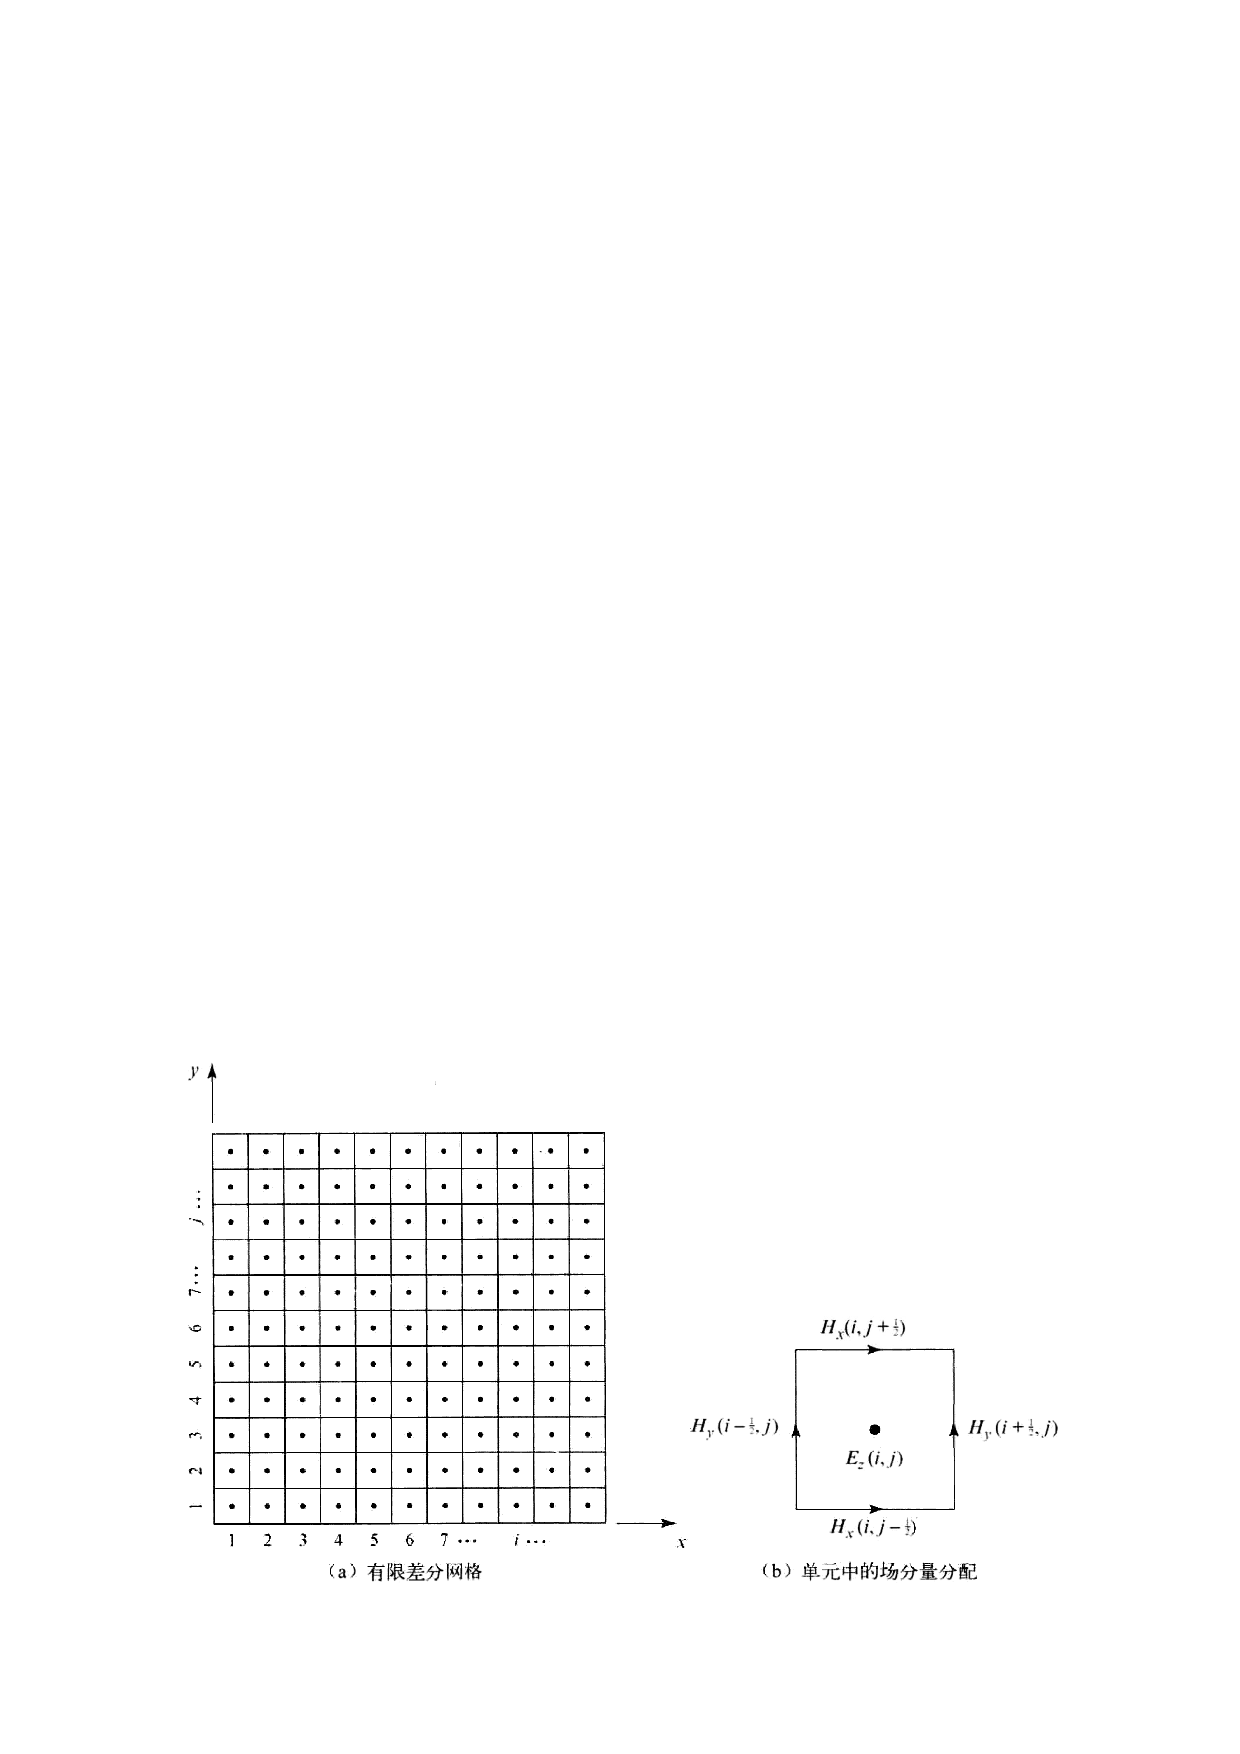
\includegraphics[scale=1]{2.4.1-1.pdf}
    \caption{Yee 网格有限差分算法}
\end{figure}

\begin{theorem}{时间步进公式}
    对于 Yee 网格,
    式 (\ref{Yee Maxwell 方程组-1}),式 (\ref{Yee Maxwell 方程组-2}) 
    和式 (\ref{Yee Maxwell 方程组-3})
    的时间步进公式分别为
    \begin{equation}
        \mathscr{H}_x^{n+\frac{1}{2}}\left(i,j+\frac{1}{2}\right)=
        \mathscr{H}_x^{n-\frac{1}{2}}\left(i,j+\frac{1}{2}\right)
        -\frac{\Delta t}{\mu \Delta y}\Big[
        \mathscr{E}_z^n(i,j+1)-\mathscr{E}_z^n(i,j)
        \Big]
        \label{Yee 时间步进公式-1}
    \end{equation}
    \begin{equation}
        \mathscr{H}_y^{n+\frac{1}{2}}\left(i+\frac{1}{2},j\right)=
        \mathscr{H}_y^{n-\frac{1}{2}}\left(i+\frac{1}{2},j\right)
        -\frac{\Delta t}{\mu \Delta y}\Big[
        \mathscr{E}_z^n(i+1,j)-\mathscr{E}_z^n(i,j)
        \Big]
        \label{Yee 时间步进公式-2}
    \end{equation}
    \begin{equation}
        \begin{aligned}
            \mathscr{E}_z^{n+1}(i,j)=&\ \frac{1}{\beta(i,j)}
            \Bigg\{\alpha(i,j)\mathscr{E}_z^n(i,j)+\frac{1}{\Delta x}\left[
                \mathscr{H}_y^{n+\frac{1}{2}}\left(i+\frac{1}{2},j\right)
                -\mathscr{H}_y^{n+\frac{1}{2}}\left(i-\frac{1}{2},j\right)
            \right]\\
            &-\frac{1}{\Delta y}
            \left[\mathscr{H}_x^{n+\frac{1}{2}}\left(i,j+\frac{1}{2}\right)
            -\mathscr{H}_x^{n+\frac{1}{2}}\left(i,j-\frac{1}{2}\right)
            \right]-\mathscr{J}_z^{n+\frac{1}{2}}(i,j)
            \Bigg\}
        \end{aligned}
        \label{Yee 时间步进公式-3}
    \end{equation}
    其中 $\alpha(i,j)=\frac{\epsilon}{\Delta t}-\frac{\sigma}{2}$,
    $\beta(i,j)=\frac{\epsilon}{\Delta t}+\frac{\sigma}{2}$。
\end{theorem}

\begin{exercise}
    推导上述方程。
\end{exercise}

\begin{solution}
    以式 (\ref{Yee Maxwell 方程组-1}) 为例,对时间采用中心差分,我们有
    \begin{equation*}
        \frac{\mathscr{E}_z^n(i,j+1)-\mathscr{E}_z^n(i,j)}{\Delta y}
        =-\mu \frac{\mathscr{H}_x^{n+\frac{1}{2}}\left(i,j+\frac{1}{2}\right)
        -\mathscr{H}_x^{n-\frac{1}{2}}\left(i,j+\frac{1}{2}\right)}{\Delta t}
    \end{equation*}
    整理得
    \begin{equation*}
        \mathscr{H}_x^{n+\frac{1}{2}}\left(i,j+\frac{1}{2}\right)=
        \mathscr{H}_x^{n-\frac{1}{2}}\left(i,j+\frac{1}{2}\right)
        -\frac{\Delta t}{\mu \Delta y}\Big[
        \mathscr{E}_z^n(i,j+1)-\mathscr{E}_z^n(i,j)
        \Big]
    \end{equation*}
\end{solution}

\par 对于给定 $\mathscr{E}_z$、$\mathscr{H}_x$ 
及 $\mathscr{H}_y$ 的初值和适当的边界条件,
可以用式 (\ref{Yee 时间步进公式-1}) 和式 (\ref{Yee 时间步进公式-2}) 计
算 $\mathscr{H}_x$ 
和 $\mathscr{H}_y$,然后用式 (\ref{Yee 时间步进公式-3}) 计算
$\mathscr{E}_z$。

\begin{note}
    Yee 网格中,场和磁场的空间网格错开
    了半个网格点,在时间采样点上也错开半个时间步。
    更重要的是,磁场分量的采样在矩形单
    元的边缘:$\mathscr{H}_x$ 在与 $x$ 平行的边缘上采样;
    $\mathscr{H}_y$ 在与 $y$ 平行的边缘上采样。这种采样方式保证
    了场的唯一定义,并且自动确保了切向场的连续性。
\end{note}

\par 基于式 (\ref{Yee 时间步进公式-1})
和式 (\ref{Yee 时间步进公式-2}) 的时间步进公式称为蛙跳时间积分。

\begin{exercise}
    从积分形式的 Maxwell 方程组出发,推导 Yee 网格的时间步进公式。
\end{exercise}

\subsection{三维分析}

\par Yee 网格有限差分算法可直接从二维扩展到三维。

\begin{definition}{三维 Maxwell 方程组}
    考虑时域 Maxwell 方程组
    \begin{align}
        \nabla \times \vec{\mathscr{E}} &= -\mu \frac{\partial \vec{\mathscr{H}}}{\partial t}\\
        \nabla \times \vec{\mathscr{H}} &= 
        \epsilon \frac{\partial \vec{\mathscr{E}}}{\partial t}
        +\sigma \vec{\mathscr{E}}
        +\vec{\mathscr{J}_i}
    \end{align}
    这两个矢量方程可以写成 6 个标量方程
    \begin{align}
        \label{Yee 三维 Maxwell 方程组-1}
        \frac{\partial \mathscr{E}_z}{\partial y}
        -\frac{\partial \mathscr{E}_y}{\partial z}
        &= -\mu \frac{\partial \mathscr{H}_x}{\partial t}\\
        \label{Yee 三维 Maxwell 方程组-2}
        \frac{\partial \mathscr{E}_x}{\partial z}
        -\frac{\partial \mathscr{E}_z}{\partial x}
        &= -\mu \frac{\partial \mathscr{H}_y}{\partial t}\\
        \label{Yee 三维 Maxwell 方程组-3}
        \frac{\partial \mathscr{E}_y}{\partial x}
        -\frac{\partial \mathscr{E}_x}{\partial y}
        &= -\mu \frac{\partial \mathscr{H}_z}{\partial t}\\
        \label{Yee 三维 Maxwell 方程组-4}
        \frac{\partial \mathscr{H}_z}{\partial y}
        -\frac{\partial \mathscr{H}_y}{\partial z}
        &= \epsilon \frac{\partial \mathscr{E}_x}{\partial t}
        +\sigma \mathscr{E}_x + \mathscr{J}_x\\
        \label{Yee 三维 Maxwell 方程组-5}
        \frac{\partial \mathscr{H}_x}{\partial z}
        -\frac{\partial \mathscr{H}_z}{\partial x}
        &= \epsilon \frac{\partial \mathscr{E}_y}{\partial t}
        +\sigma \mathscr{E}_y + \mathscr{J}_y\\
        \label{Yee 三维 Maxwell 方程组-6}
        \frac{\partial \mathscr{H}_y}{\partial x}
        -\frac{\partial \mathscr{H}_x}{\partial y}
        &= \epsilon \frac{\partial \mathscr{E}_z}{\partial t}
        +\sigma \mathscr{E}_z + \mathscr{J}_z
    \end{align}
\end{definition}

\par 用一个立方体包围体积 $V$,再把这
个立方体盒子分成许多小立方体单元。然后,在单元每条边的中心位置
对电场分量采样,在单元每个面的中心位置对磁场分量采样。

\begin{figure}[!htbp]
    \centering
    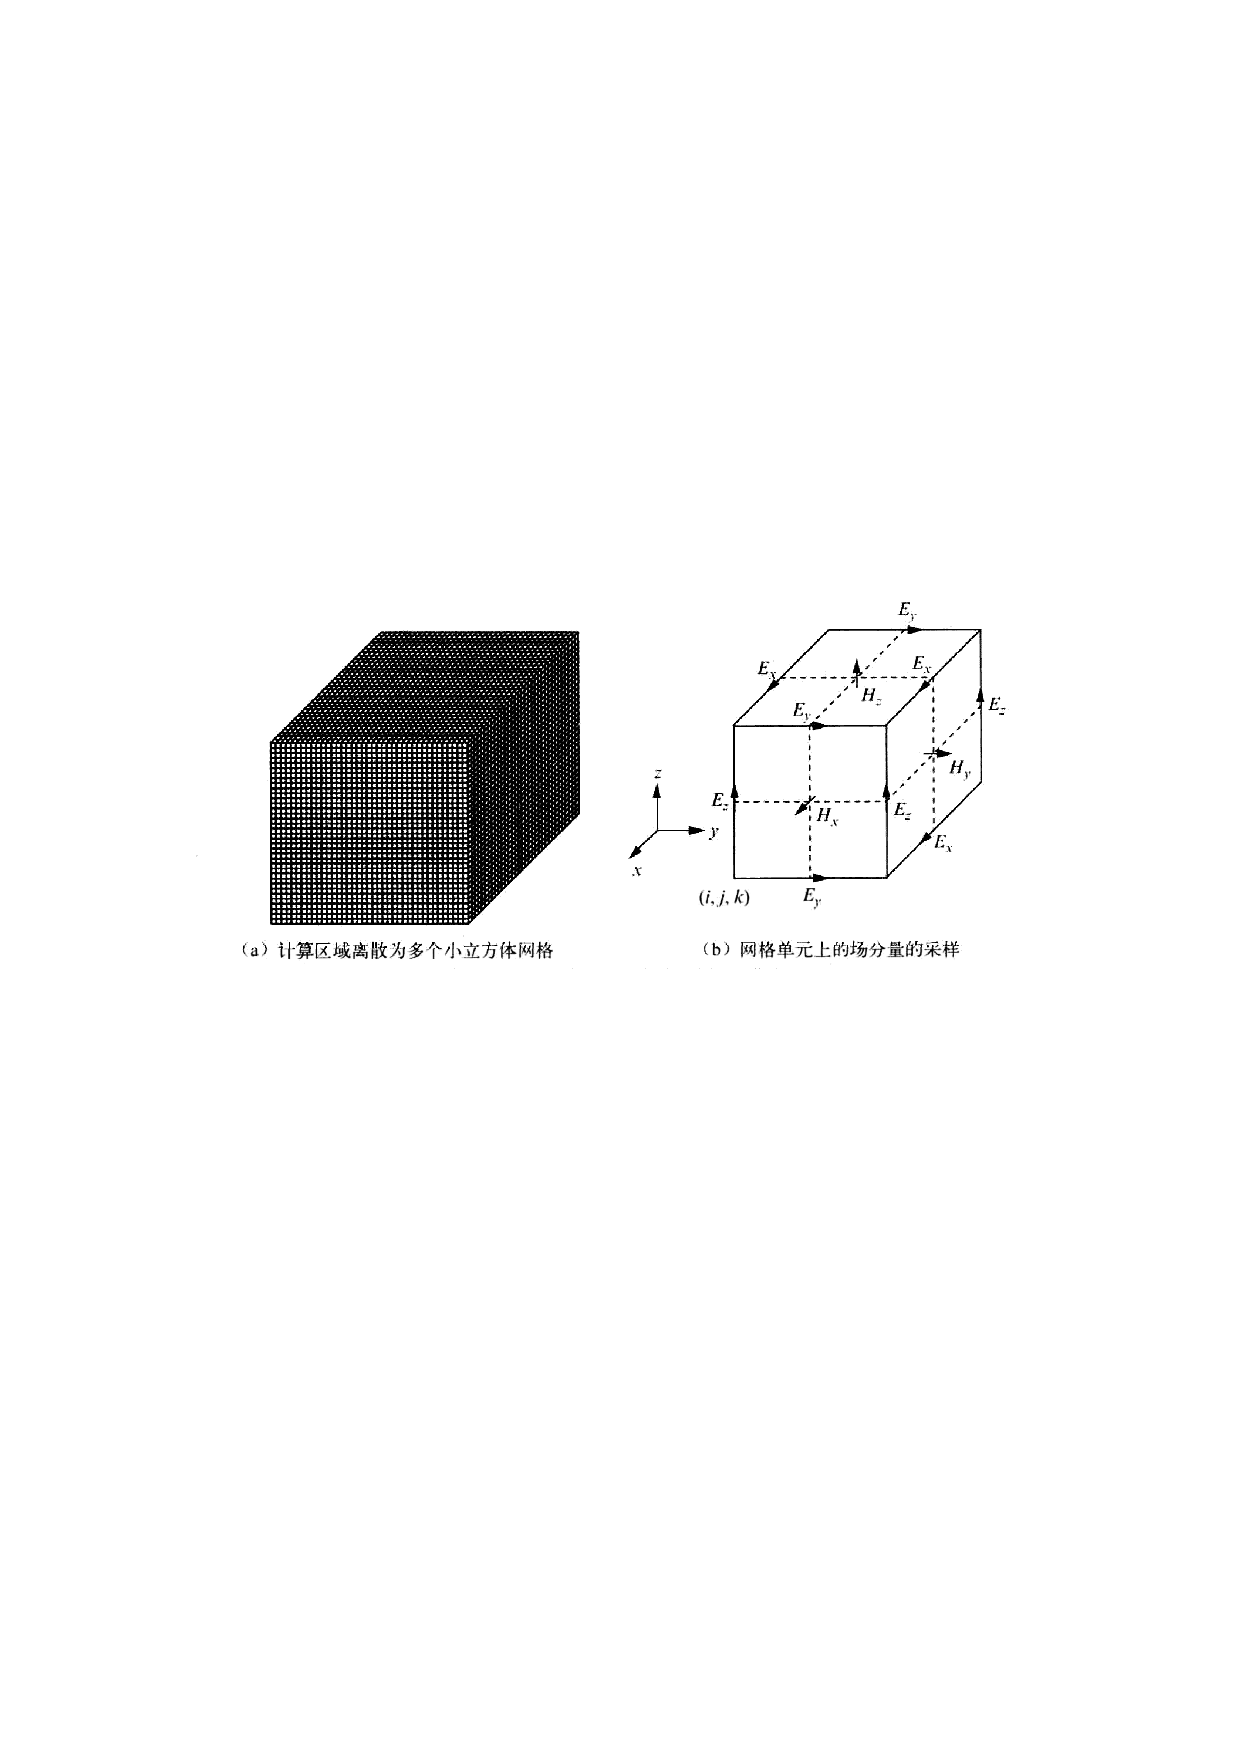
\includegraphics[scale=1]{2.4.2-1.pdf}
    \caption{Yee 网格有限差分算法}
\end{figure}

\begin{theorem}{时间步进公式}
    对于 Yee 网格,
    式 (\ref{Yee 三维 Maxwell 方程组-1})
    到式 (\ref{Yee 三维 Maxwell 方程组-6})
    的时间步进公式分别为
    \begin{equation}
        \begin{aligned}
            \mathscr{H}_x^{n+\frac{1}{2}}\left(i,j+\frac{1}{2},k+\frac{1}{2}\right)=
            &\ \mathscr{H}_x^{n-\frac{1}{2}}\left(i,j+\frac{1}{2},k+\frac{1}{2}\right)\\
            &-\frac{\Delta t}{\mu \Delta y}\left[
                \mathscr{E}_z^n\left(i,j+1,k+\frac{1}{2}\right)
                -\mathscr{E}_z^n\left(i,j,k+\frac{1}{2}\right)
            \right]\\
            &+\frac{\Delta t}{\mu \Delta z}\left[
                \mathscr{E}_y^n\left(i,j+\frac{1}{2},k+1\right)
                -\mathscr{E}_y^n\left(i,j+\frac{1}{2},k\right)
            \right]
        \end{aligned}
        \label{Yee 三维时间步进公式-1}
    \end{equation}
    \begin{equation}
        \begin{aligned}
            \mathscr{H}_y^{n+\frac{1}{2}}\left(i+\frac{1}{2},j,k+\frac{1}{2}\right)=
            &\ \mathscr{H}_y^{n-\frac{1}{2}}\left(i+\frac{1}{2},j,k+\frac{1}{2}\right)\\
            &-\frac{\Delta t}{\mu \Delta z}\left[
                \mathscr{E}_x^n\left(i+\frac{1}{2},j,k+1\right)
                -\mathscr{E}_x^n\left(i\frac{1}{2},j,k\right)
            \right]\\
            &+\frac{\Delta t}{\mu \Delta x}\left[
                \mathscr{E}_z^n\left(i+1,j,k+\frac{1}{2}\right)
                -\mathscr{E}_z^n\left(i,j,k+\frac{1}{2}\right)
            \right]
        \end{aligned}
        \label{Yee 三维时间步进公式-2}
    \end{equation}
    \begin{equation}
        \begin{aligned}
            \mathscr{H}_z^{n+\frac{1}{2}}\left(i+\frac{1}{2},j+\frac{1}{2},k\right)=
            &\ \mathscr{H}_z^{n-\frac{1}{2}}\left(i+\frac{1}{2},j+\frac{1}{2},k\right)\\
            &-\frac{\Delta t}{\mu \Delta x}\left[
                \mathscr{E}_y^n\left(i+1,j+\frac{1}{2},k\right)
                -\mathscr{E}_y^n\left(i,j+\frac{1}{2},k\right)
            \right]\\
            &+\frac{\Delta t}{\mu \Delta y}\left[
                \mathscr{E}_x^n\left(i+\frac{1}{2},j+1,k\right)
                -\mathscr{E}_x^n\left(i+\frac{1}{2},j,k\right)
            \right]
        \end{aligned}
        \label{Yee 三维时间步进公式-3}
    \end{equation}
    \begin{equation}
        \begin{aligned}
            \mathscr{E}_x^{n+1}\left(i+\frac{1}{2},j,k\right)=
            &\ \frac{1}{\beta\left(i+\frac{1}{2},j,k\right)}
            \Bigg\{\alpha\left(i+\frac{1}{2},j,k\right)
            \mathscr{E}_x^n\left(i+\frac{1}{2},j,k\right)\\
            &+\frac{1}{\Delta y}\left[
                \mathscr{H}_z^{n+\frac{1}{2}}\left(i+\frac{1}{2},j+\frac{1}{2},k\right)
                -\mathscr{H}_z^{n+\frac{1}{2}}\left(i+\frac{1}{2},j-\frac{1}{2},k\right)
            \right]\\
            &-\frac{1}{\Delta z}\left[
                \mathscr{H}_y^{n+\frac{1}{2}}\left(i+\frac{1}{2},j,k+\frac{1}{2}\right)
                -\mathscr{H}_y^{n+\frac{1}{2}}\left(i+\frac{1}{2},j,k-\frac{1}{2}\right)
            \right]\\
            &-\mathscr{J}_x^{n+\frac{1}{2}}\left(i+\frac{1}{2},j,k\right)
            \Bigg\}
        \end{aligned}
        \label{Yee 三维时间步进公式-4}
    \end{equation}
    \begin{equation}
        \begin{aligned}
            \mathscr{E}_y^{n+1}\left(i,j+\frac{1}{2},k\right)=
            &\ \frac{1}{\beta\left(i,j+\frac{1}{2},k\right)}
            \Bigg\{\alpha\left(i,j+\frac{1}{2},k\right)
            \mathscr{E}_y^n\left(i,j+\frac{1}{2},k\right)\\
            &+\frac{1}{\Delta z}\left[
                \mathscr{H}_x^{n+\frac{1}{2}}\left(i,j+\frac{1}{2},k+\frac{1}{2}\right)
                -\mathscr{H}_x^{n+\frac{1}{2}}\left(i,j+\frac{1}{2},k-\frac{1}{2}\right)
            \right]\\
            &-\frac{1}{\Delta x}\left[
                \mathscr{H}_z^{n+\frac{1}{2}}\left(i+\frac{1}{2},j+\frac{1}{2},k\right)
                -\mathscr{H}_z^{n+\frac{1}{2}}\left(i-\frac{1}{2},j+\frac{1}{2},k\right)
            \right]\\
            &-\mathscr{J}_y^{n+\frac{1}{2}}\left(i,j+\frac{1}{2},k\right)
            \Bigg\}
        \end{aligned}
        \label{Yee 三维时间步进公式-5}
    \end{equation}
    \begin{equation}
        \begin{aligned}
            \mathscr{E}_z^{n+1}\left(i,j,k+\frac{1}{2}\right)=
            &\ \frac{1}{\beta\left(i,j,k+\frac{1}{2}\right)}
            \Bigg\{\alpha\left(i,j,k+\frac{1}{2}\right)
            \mathscr{E}_z^n\left(i,j,k+\frac{1}{2}\right)\\
            &+\frac{1}{\Delta x}\left[
                \mathscr{H}_y^{n+\frac{1}{2}}\left(i+\frac{1}{2},j,k+\frac{1}{2}\right)
                -\mathscr{H}_y^{n+\frac{1}{2}}\left(i-\frac{1}{2},j,k+\frac{1}{2}\right)
            \right]\\
            &-\frac{1}{\Delta y}\left[
                \mathscr{H}_x^{n+\frac{1}{2}}\left(i,j+\frac{1}{2},k+\frac{1}{2}\right)
                -\mathscr{H}_x^{n+\frac{1}{2}}\left(i,j-\frac{1}{2},k+\frac{1}{2}\right)
            \right]\\
            &-\mathscr{J}_z^{n+\frac{1}{2}}\left(i,j,k+\frac{1}{2}\right)
            \Bigg\}
        \end{aligned}
        \label{Yee 三维时间步进公式-6}
    \end{equation}
    其中 $\alpha(i,j)=\frac{\epsilon}{\Delta t}-\frac{\sigma}{2}$,
    $\beta(i,j)=\frac{\epsilon}{\Delta t}+\frac{\sigma}{2}$。
\end{theorem}

\begin{exercise}
    推导上述方程。
\end{exercise}

\begin{exercise}
    从积分形式的 Maxwell 方程组出发,推导 Yee 网格的时间步进公式。
\end{exercise}

\par 给定源电流、电场和磁场的初始值及边界条件,使用
式 (\ref{Yee 三维时间步进公式-1}) 至
式 (\ref{Yee 三维时间步进公式-3}) 计算下一个时间步的
磁场,然后用
式 (\ref{Yee 三维时间步进公式-4}) 至
式 (\ref{Yee 三维时间步进公式-6}) 计算下一个时间步的电
场。

\begin{theorem}{稳定性条件}
    保证时间步进的稳定性,其时间步长应满足稳定性条件
    \begin{equation}
        \Delta t \leq \frac{\sqrt{\mu \epsilon}}
        {\sqrt{\frac{1}{(\Delta x)^2}+\frac{1}{(\Delta y)^2}+\frac{1}{(\Delta z)^2}}}
    \end{equation}
\end{theorem}

\begin{theorem}{三维数值色散}
    将数值色散误差公式拓展到三维情况,其表达式为
    \begin{equation}
        \frac{\tilde{k}-k}{k}
        \approx\frac{1}{24}
        \Bigg\{
            \Big[
                (k\Delta x)^2\cos^4\phi^i
                +(k\Delta y)^2\sin^4\phi^i
            \Big]\sin^4\theta^i
            +(k\Delta z)^2\cos^4\theta^i
            -(\omega \Delta t)^2
        \Bigg\}
    \end{equation}
    其中 $(\phi^i,\theta^i)$ 表示波的传播方向。
\end{theorem}

\begin{example}
    若选择 $\Delta x=\Delta y=\Delta z = h$ 和 $\Delta t = \frac{0.5h}{c}$,则数值相位误差为
    \begin{equation*}
        \begin{aligned}
            \frac{\tilde{k}-k}{k}
            &\approx\frac{(kh)^2}{24}
            \Bigg\{
                \Big[
                    \cos^4\phi^i
                    +\sin^4\phi^i
                \Big]\sin^4\theta^i
                +\cos^4\theta^i
                -\frac{1}{4}
            \Bigg\}\\
            &=\frac{\pi^2}{6}\left(\frac{h}{\lambda}\right)^2
            \Bigg\{
                \Big[
                    \cos^4\phi^i
                    +\sin^4\phi^i
                \Big]\sin^4\theta^i
                +\cos^4\theta^i
                -\frac{1}{4}
            \Bigg\}
        \end{aligned}
    \end{equation*}
\end{example}

\section{吸收边界条件}

\par 使用有限差分法求解无界电磁问题时需要将无限的计算
空间截断成有限的计算区域。

\subsection{一维吸收边界条件}

\par 假定求解区域
无界 $-\infty<x<\infty$,
但源限定在有限的区域内 $(a\leq x \leq b)$。
该源将在 $x>b$ 区域产生沿 $x$ 正方向
传播的波,在 $x<a$ 区域产生沿 $x$ 负方向传播的波。
\par 使用有限差分求解这个问题,我们将无
限求解区域截断为有限区域 $[A,B]$,
其中 $A<a$ 且 $B>b$。
我们希望建立一个边界条
件,使得波能透过 $x=A$ 和 $x=B$ 这两个人为设置的截断面而没有任何反射。

\begin{theorem}{一维吸收边界条件}{一维吸收边界条件}
    以 $x=B$ 点为例,一维吸收边界条件为
    \begin{equation}
        \frac{\partial \mathscr{E}_z(x,t)}{\partial x}
        =-\frac{1}{c}\frac{\partial \mathscr{E}_z(x,t)}{\partial t}
    \end{equation}
\end{theorem}

\begin{exercise}
    证明上述公式。
\end{exercise}

\begin{solution}
    在 $x=B$ 处,波向 $x$ 正方向传播,其频域方程为
    \begin{equation*}
        E_z(x)=E_0e^{-jkx}
    \end{equation*}
    其中,$E_0$ 为未知量,$k=\omega\sqrt{\mu \epsilon}$,对其求导得
    \begin{equation*}
        \frac{\partial E_z(x)}{\partial x}=-jkE_0e^{-jkx}=-jkE_z(x)
        =-\frac{j\omega}{c}E_z(x)
    \end{equation*}
    作 Fourier 逆变换,得到
    \begin{equation*}
        \frac{\partial \mathscr{E}_z(x,t)}{\partial x}
        =-\frac{1}{c}\frac{\partial \mathscr{E}_z(x,t)}{\partial t}
    \end{equation*}
\end{solution}

\begin{theorem}{边界时间步进公式}
    以 $x=B$ 点为例,使用后向差分离散对 $x$ 的导数,而使用前向差分离散对 $t$ 的导数,得到
    \begin{equation}
        \mathscr{E}_z^{n+1}(M)=\mathscr{E}_z^{n}(M)
        -\frac{c\Delta t}{\Delta x}
        \Big[\mathscr{E}_z^{n}(M)-\mathscr{E}_z^{n}(M-1)\Big]
    \end{equation}
    其稳定性条件为 $\Delta t \leq \frac{\Delta x}{c}$。
\end{theorem}

\begin{exercise}
    证明上述公式。
\end{exercise}

\begin{solution}
    由定理 \ref{thm:一维吸收边界条件},我们有
    \begin{equation*}
        \frac{\partial \mathscr{E}_z(x,t)}{\partial x}
        =-\frac{1}{c}\frac{\partial \mathscr{E}_z(x,t)}{\partial t}
    \end{equation*}
    使用后向差分离散对 $x$ 的导数,而使用前向差分离散对 $t$ 的导数,得到
    \begin{equation*}
        \frac{\mathscr{E}_z^{n}(M)-\mathscr{E}_z^{n}(M-1)}{\Delta x}
        =-\frac{1}{c}\frac{\mathscr{E}_z^{n+1}(M)-\mathscr{E}_z^{n}(M)}{\Delta t}
    \end{equation*}
    整理得
    \begin{equation*}
        \mathscr{E}_z^{n+1}(M)=\mathscr{E}_z^{n}(M)
        -\frac{c\Delta t}{\Delta x}
        \Big[\mathscr{E}_z^{n}(M)-\mathscr{E}_z^{n}(M-1)\Big]
    \end{equation*}
\end{solution}

\begin{theorem}{边界时间步进公式}
    以 $x=B$ 点为例,使用中心差分离散对 $x$ 和 $t$ 的导数,得到
    \begin{equation}
        \mathscr{E}_z^{n+1}(M)=\mathscr{E}_z^{n}(M-1)
        -\frac{\Delta x-c\Delta t}{\Delta x + c\Delta t}
        \Big[\mathscr{E}_z^{n}(M)-\mathscr{E}_z^{n+1}(M-1)\Big]
    \end{equation}
    此式是无条件稳定的。
\end{theorem}

\begin{exercise}
    证明上述公式。
\end{exercise}

\begin{solution}
    由定理 \ref{thm:一维吸收边界条件},我们有
    \begin{equation*}
        \frac{\partial \mathscr{E}_z(x,t)}{\partial x}
        =-\frac{1}{c}\frac{\partial \mathscr{E}_z(x,t)}{\partial t}
    \end{equation*}
    在 $x=\left(M-\frac{1}{2}\right)\Delta x$ 和
    $t=\left(n+\frac{1}{2}\right)\Delta t$ 处采用具有二阶精度的中心差分,得到
    \begin{equation*}
        \frac{\mathscr{E}_z^{n+\frac{1}{2}}(M)-\mathscr{E}_z^{n+\frac{1}{2}}(M-1)}{\Delta x}
        =-\frac{1}{c}\frac{\mathscr{E}_z^{n+1}\left(M-\frac{1}{2}\right)-\mathscr{E}_z^{n}\left(M-\frac{1}{2}\right)}{\Delta t}
    \end{equation*}
    使用场值在半网格点及半时间步的平均值,可以得到二阶精度的时间步进公式
    \begin{equation*}
        \frac{1}{2}\left(
            \frac{\mathscr{E}_z^{n+1}(M)-\mathscr{E}_z^{n+1}(M-1)}{\Delta x}
            +\frac{\mathscr{E}_z^{n}(M)-\mathscr{E}_z^{n}(M-1)}{\Delta x}
        \right)
        =-\frac{1}{c}\frac{1}{2}
        \left(
            \frac{\mathscr{E}_z^{n+1}(M-1)-\mathscr{E}_z^{n}(M-1)}{\Delta t}
            +\frac{\mathscr{E}_z^{n+1}(M)-\mathscr{E}_z^{n}(M)}{\Delta t}
        \right)
    \end{equation*}
    整理得
    \begin{equation*}
        \mathscr{E}_z^{n+1}(M)=\mathscr{E}_z^{n}(M-1)
        -\frac{\Delta x-c\Delta t}{\Delta x + c\Delta t}
        \Big[\mathscr{E}_z^{n}(M)-\mathscr{E}_z^{n+1}(M-1)\Big]
    \end{equation*}
\end{solution}

\subsection{二维吸收边界条件}

\par 考虑在沿 $y$ 轴方向的边界上,有一个平面波入射到此边
界,表示为
\begin{equation}
    \varphi(x,y)=Ae^{-j(k_x x+k_y y)}
\end{equation}

\begin{theorem}{二维吸收边界条件}{二维吸收边界条件}
    在频域中,二维吸收边界条件为
    \begin{equation}
        \frac{\partial \varphi}{\partial x}
        =-jk_xAe^{-j(k_x x+k_y y)}
        =-jk_x\varphi
        =-jk\cos \theta \varphi
        \label{二维精确吸收边界条件}
    \end{equation}
\end{theorem}

\par 定理 \ref{thm:二维吸收边界条件} 中给出的边界条件可以完全吸
收与 $x$ 轴成 $\theta$ 角入射的平面波。然而,对于一般的问题,入
射到吸收边界的通常不是平面波,并且入射角通常是未知
的。因此,一个实际可用的边界条件必须与入射角无关。

\begin{theorem}{一阶吸收边界条件}{一阶吸收边界条件}
    若在式 (\ref{二维精确吸收边界条件}) 中设 $\theta=0$,则得到一个近似的边界条件为
    \begin{equation}
        \frac{\partial \varphi}{\partial x}
        \approx-jk\varphi
        \label{一阶频域吸收边界条件}
    \end{equation}
    这种边界条件对应的反射系数为
    \begin{equation}
        R=\frac{\cos \theta -1}{\cos \theta +1}
    \end{equation}
\end{theorem}

\begin{theorem}{二阶吸收边界条件}{二阶吸收边界条件}
    二阶吸收边界条件为
    \begin{equation}
        \frac{\partial \varphi}{\partial x}
        \approx-jk\varphi
        -\frac{j}{2k}\frac{\partial^2 \varphi}{\partial y^2}
        \label{二阶频域吸收边界条件}
    \end{equation}
    这种边界条件对应的反射系数为
    \begin{equation}
        R=\frac{\cos \theta +\frac{1}{2}\sin^2\theta-1}
        {\cos \theta -\frac{1}{2}\sin^2\theta+1}
    \end{equation}
\end{theorem}

\begin{exercise}
    证明上述公式。
\end{exercise}

\begin{solution}
    将式 (\ref{二维精确吸收边界条件}) 重写为
    \begin{equation*}
        \frac{\partial \varphi}{\partial x}
        =-jk_x\varphi
        =-j\sqrt{k^2-k_y^2}\varphi
        =-jk\sqrt{1-\left(\frac{k_y}{k}\right)^2}\varphi
    \end{equation*}
    将 $\sqrt{1-\left(\frac{k_y}{k}\right)^2}$ 作 Taylor 展开,保留前两项,得到
    \begin{equation*}
        \frac{\partial \varphi}{\partial x}
        \approx -jk\left[
            1-\frac{1}{2}\left(\frac{k_y}{k}\right)^2
        \right]\varphi
        =-jk\varphi+\frac{j}{2k}k_y^2\varphi
    \end{equation*}
    由于 $\frac{\partial^2 \varphi}{\partial y^2}=-k_y^2\varphi$,上式可写为
    \begin{equation*}
        \frac{\partial \varphi}{\partial x}
        \approx -jk\varphi-\frac{j}{2k}\frac{\partial^2 \varphi}{\partial y^2}
    \end{equation*}
\end{solution}

\begin{exercise}
    证明上述公式。
\end{exercise}

\begin{theorem}{Engquist-Majda 吸收边界条件}
    将定理 \ref{thm:二阶吸收边界条件} 中的边界条件转化到时域,得到
    \begin{equation}
        \frac{\partial^2 \varphi}{\partial t \partial x}
        \approx -\frac{1}{c}
        \frac{\partial^2 \varphi}{\partial t^2}
        +\frac{c}{2}\frac{\partial^2 \varphi}{\partial y^2}
        \label{二阶时域吸收边界条件}
    \end{equation}
\end{theorem}

\begin{exercise}
    证明上述公式。
\end{exercise}

\begin{solution}
    将式 (\ref{二阶频域吸收边界条件}) 中的边界条件转化到时域,
    首先用 $k=\frac{\omega}{c}$ 将其重写
    \begin{align*}
        \frac{\partial \varphi}{\partial x}
        &\approx-j\frac{\omega}{c}\varphi
        -\frac{jc}{2\omega}\frac{\partial^2 \varphi}{\partial y^2}\\
        j\omega\frac{\partial \varphi}{\partial x}
        &\approx\frac{\omega^2}{c}\varphi
        +\frac{c}{2}\frac{\partial^2 \varphi}{\partial y^2}
    \end{align*}
    作 Fourier 逆变换,得到
    \begin{equation*}
        \frac{\partial^2 \varphi}{\partial t \partial x}
        \approx -\frac{1}{c}
        \frac{\partial^2 \varphi}{\partial t^2}
        +\frac{c}{2}\frac{\partial^2 \varphi}{\partial y^2}
    \end{equation*}
\end{solution}

\begin{theorem}{边界时间步进公式}
    对式 (\ref{二阶时域吸收边界条件}) 
    左边使用前向差分离散,右边使用中心差分离散,得到
    \begin{equation}
        \begin{aligned}
            \varphi^{n+1}(M,j)=
            &\ \left[\frac{1}{\Delta x\Delta t}+\frac{1}{c(\Delta t)^2}\right]^{-1}
            \Bigg\{
                \frac{1}{\Delta x\Delta t}\Big[
                    \varphi^{n+1}(M-1,j)-\varphi^{n}(M-1,j)
                \Big]\\
            &+\left[
                \frac{1}{\Delta x\Delta t}
                +\frac{2}{c(\Delta t)^2}
                -\frac{c}{(\Delta y)^2}
            \right]\varphi^{n}(M,j)
            -\frac{1}{c(\Delta t)^2}\varphi^{n-1}(M,j)\\
            &+\frac{c}{2(\Delta y)^2}\Big[
                \varphi^{n}(M,j-1)+\varphi^{n}(M,j+1)
            \Big]
            \Bigg\}
        \end{aligned}
    \end{equation}
\end{theorem}

\subsection{理想匹配层}

\begin{definition}{修正 Maxwell 方程}
    考虑无源情况下的修正 Maxwell 方程
    \begin{align}
        \nabla_s\times\vec{E}&=-j\omega\mu\vec{H}\\
        \nabla_s\times\vec{H}&=j\omega\epsilon\vec{E}\\
        \nabla_s\cdot(\epsilon\vec{E})&=0\\
        \nabla_s\cdot(\mu\vec{H})&=0
    \end{align}
    其中,$\nabla_s$ 定义为
    \begin{equation}
        \nabla_s=
        \vec{x}\frac{1}{s_x}\frac{\partial}{\partial x}
        +\vec{y}\frac{1}{s_y}\frac{\partial}{\partial y}
        +\vec{z}\frac{1}{s_z}\frac{\partial}{\partial z}
    \end{equation}
    $\nabla_s$ 可认为是 $x$、$y$ 和 $z$ 轴
    分别被 $s_x$、$s_y$ 和 $s_z$ 因子拉伸的
    的 $\nabla$ 算子。
\end{definition}

\begin{theorem}{色散关系}
    满足修正 Maxwell 方程组的电磁波的色散关系为
    \begin{equation}
        \left(
            \frac{k_x}{s_x}
        \right)^2
        +\left(
            \frac{k_y}{s_y}
        \right)^2
        +\left(
            \frac{k_z}{s_z}
        \right)^2=k^2
    \end{equation}
    此方程的解为
    \begin{equation}
        \left\{
            \begin{aligned}
                k_x&=k s_x\sin \theta \cos \phi\\
                k_y&=k s_y\sin \theta \sin \phi\\
                k_z&=k s_z\cos \theta
            \end{aligned}
        \right.
    \end{equation}
\end{theorem}

\begin{exercise}
    证明上述公式。
\end{exercise}

\begin{solution}
    考虑一个平面波,其电场和磁场分别为
    \begin{align*}
        \vec{E}&=\vec{E}_0e^{-j\vec{k}\cdot\vec{r}}
        =\vec{E}_0e^{-j(k_x x+k_y y+k_z z)}\\
        \vec{H}&=\vec{H}_0e^{-j\vec{k}\cdot\vec{r}}
        =\vec{H}_0e^{-j(k_x x+k_y y+k_z z)}
    \end{align*}
    将上述电场和磁场代入修正 Maxwell 方程组,得到
    \begin{align*}
        \vec{k}_s\times\vec{E}&=\omega\mu\vec{H}\\
        \vec{k}_s\times\vec{H}&=-\omega\epsilon\vec{E}\\
        \vec{k}_s\cdot\vec{E}&=0\\
        \vec{k}_s\cdot\vec{H}&=0
    \end{align*}
    其中
    \begin{equation*}
        \vec{k}_s=\vec{x}\frac{k_x}{s_x}
        +\vec{y}\frac{k_y}{s_y}
        +\vec{z}\frac{k_z}{s_z}
    \end{equation*}
    将 $\vec{k}_s\times\vec{E}=\omega\mu\vec{H}$ 
    两边叉乘 $\vec{k}_s$,得到
    \begin{equation*}
        \vec{k}_s\times(\vec{k}_s\times\vec{E})
        =\omega\mu\vec{k}_s\times\vec{H}
        =-\omega^2\mu\epsilon\vec{E}
    \end{equation*}
    由于 $\vec{k}_s\times(\vec{k}_s\times\vec{E})=
    \vec{k}_s(\vec{k}_s\cdot\vec{E})
    -(\vec{k}_s\cdot\vec{k}_s)\vec{E}$
    以及 $\vec{k}_s\cdot\vec{E}=0$,上式变为
    \begin{equation*}
        (\vec{k}_s\cdot\vec{k}_s)\vec{E}
        =\omega^2\epsilon\mu\vec{E}
    \end{equation*}
    由此得到色散关系式为
    \begin{equation*}
        \vec{k}_s\cdot\vec{k}_s
        =\omega^2\epsilon\mu=k^2
    \end{equation*}
    代入 $\vec{k}_s$ 的表达式,得到
    \begin{equation*}
        \left(
            \frac{k_x}{s_x}
        \right)^2
        +\left(
            \frac{k_y}{s_y}
        \right)^2
        +\left(
            \frac{k_z}{s_z}
        \right)^2=k^2
    \end{equation*}
\end{solution}

\par 接着考虑电磁波在拉伸坐标系中两个半空间分界
面处的反射情况。

\begin{theorem}{反射系数}
    对于 $\text{TE}_z$ 入射的情况,
    使用相位匹配条件及 $\vec{E}$ 与 $\vec{H}$ 的切向分量连续条件,可以得到
    \begin{equation}
        R_{\text{TE}}
        =\frac{k_{1z}s_{2z}\mu_2-k_{2z}s_{1z}\mu_1}
        {k_{1z}s_{2z}\mu_2+k_{2z}s_{1z}\mu_1}
    \end{equation}
    其中,下标 1 表示上半空间的媒质参数,
    下标 2 表示下半空间的媒质参数。
    类似地,可以得
    到 $\text{TM}_z$ 入射时的反射系数为
    \begin{equation}
        R_{\text{TM}}
        =\frac{k_{1z}s_{2z}\epsilon_2-k_{2z}s_{1z}\epsilon_1}
        {k_{1z}s_{2z}\epsilon_2+k_{2z}s_{1z}\epsilon_1}
    \end{equation}
\end{theorem}

\begin{theorem}{理想匹配分界面}
    若选择 $\epsilon_1=\epsilon_2$、
    $\mu_1=\mu_2$、
    $s_{1x}=s_{2x}$ 以及 $s_{1y}=s_{2y}$,可以得到
    \begin{equation}
        R_{\text{TE}}=0
        \qquad
        R_{\text{TM}}=0
    \end{equation}
    上式在以下任何情形下均成立
    \begin{itemize}
        \item 任意的 $s_{1z}$ 和 $s_{2z}$
        \item 任意的 $\theta$ 和 $\phi$
        \item 任意的频率
    \end{itemize}
\end{theorem}

\begin{exercise}
    证明上述定理。
\end{exercise}

\par 由于位于 $xOy$ 平面的理想匹配分界面
与 $s_{1z}$ 和 $s_{2z}$ 无关,选择任意的 $s_{1z}$ 
和 $s_{2z}$ 均不会引起任何反射。
\par 如果选择 $s_{2z}=s'-js''$,
其中 $s'$ 和 $s''$ 是实数,
且有 $s'\geq1$和 $s''\geq0$,
则 $k_{2z}=k_2(s'-js'')\cos 0$。
因此,透射波将在负 $z$ 方向指数衰减。
若我们将媒质 2 截断成厚度为 $L$ 的
介质层,并在其后放置一块导电平面,则其反射系数的幅度变为
\begin{equation}
    |R(\theta)|=e^{-2k_2\cos \theta \int_{0}^{L}s''(z) \text{d}z}
\end{equation}

\begin{figure}[!htbp]
    \centering
    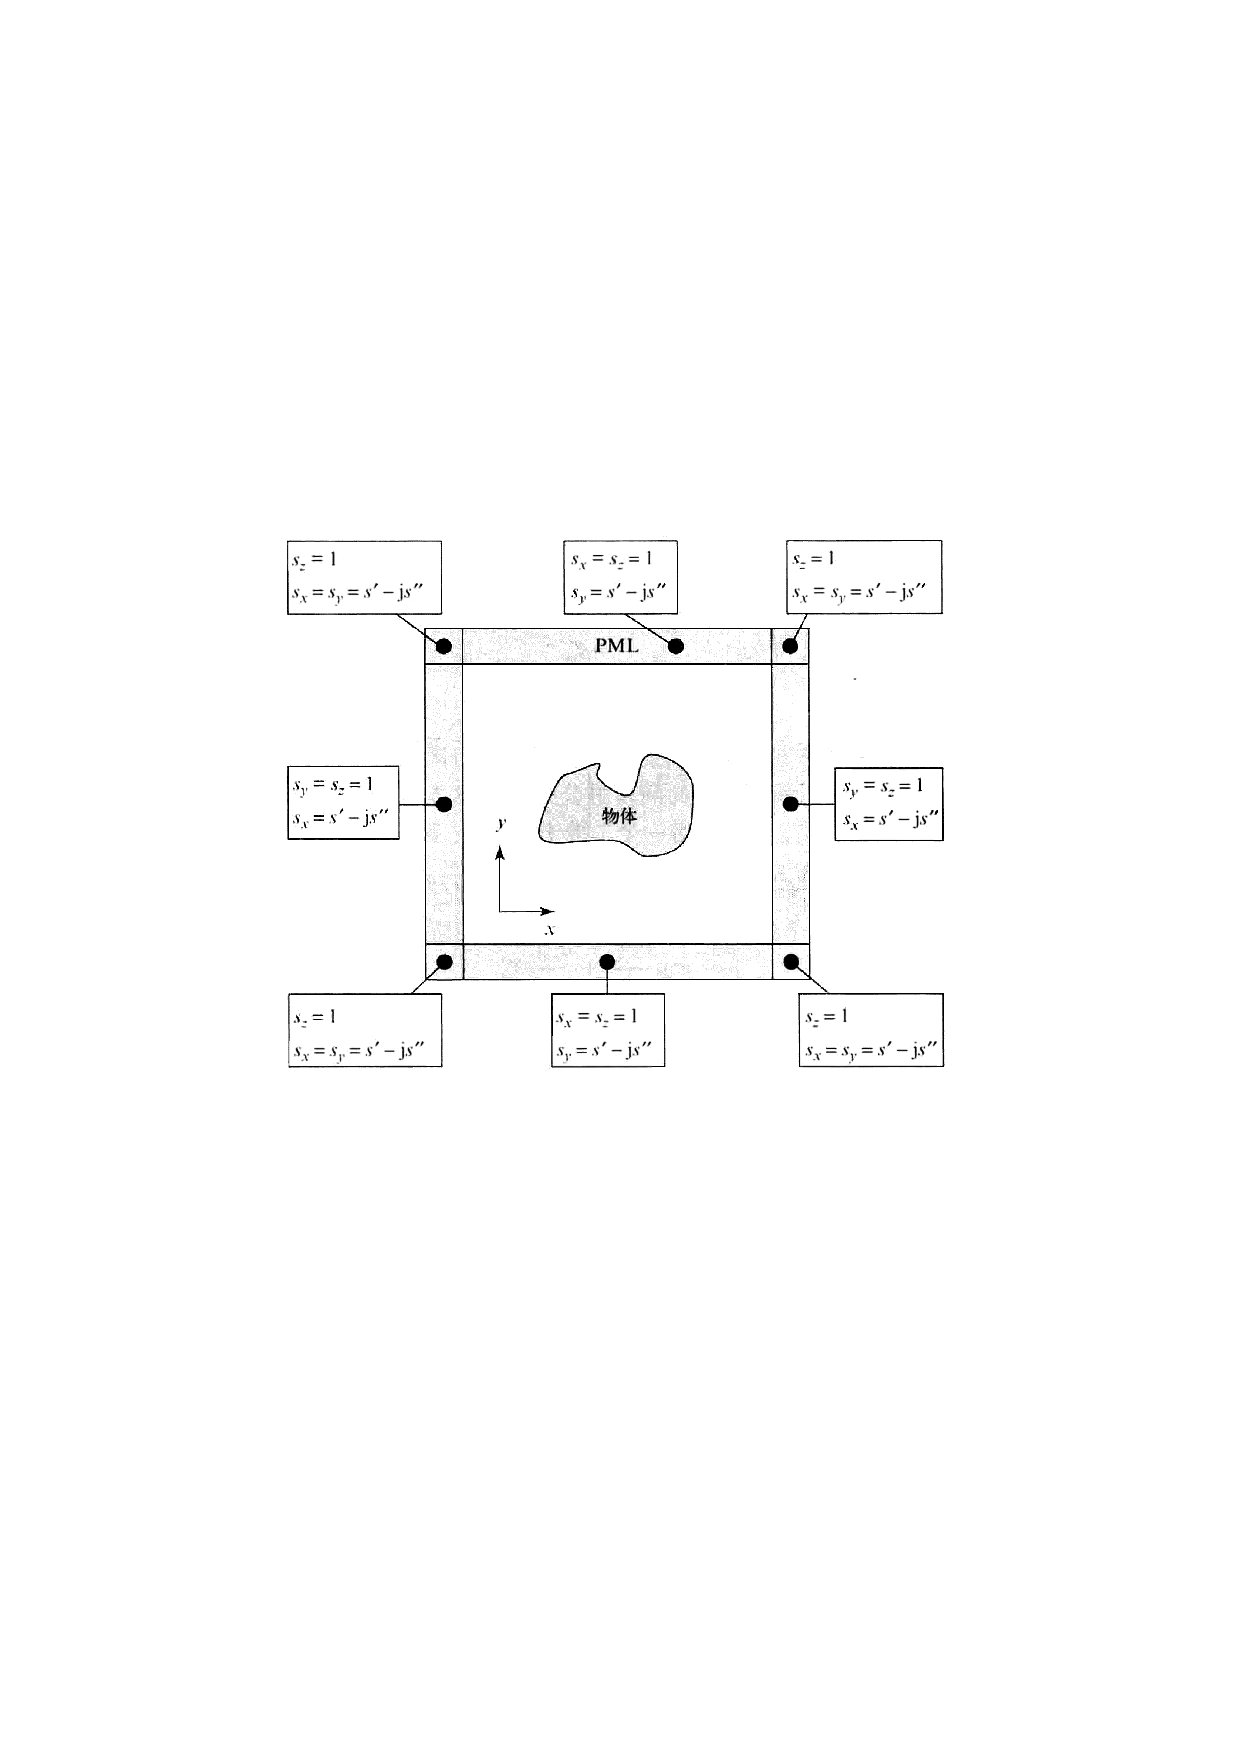
\includegraphics[scale=1]{2.5.3-1.pdf}
    \caption{采用以导电面为衬底的理想匹配层截断计算区域}
\end{figure}

\section{色散媒质的模拟}

\par 实际应用中的许多媒质是有色散的,
通常有两种方法对色散媒质进行模拟。

\subsection{递归卷积法}

\par 考虑 Maxwell 方程组中的 Maxwell-Ampere 定律
\begin{equation}
    \nabla \times \vec{\mathscr{H}}=
    \frac{\partial \vec{\mathscr{D}}}{\partial t}
    +\sigma \mathscr{E}
\end{equation}
\par 对于色散媒质,
我们最关心的是如何计算 $\frac{\partial \vec{\mathscr{D}}}{\partial t}$
这一项。

\begin{definition}{本构关系}{电色散媒质的本构关系}
    考虑一种电色散媒质,其
    电通密度 $\vec{\mathscr{D}}(t)$ 与
    电场强度 $\vec{\mathscr{E}}(t)$ 的本构关系为
    \begin{equation}
        \begin{aligned}
            \vec{\mathscr{D}}(t)
            &=\epsilon_{\infty}\vec{\mathscr{E}}(t)
            +\epsilon_0 \chi_{\text{e}}(t) * \vec{\mathscr{E}}(t)\\
            &=\epsilon_{\infty}\vec{\mathscr{E}}(t)
            +\epsilon_0 \int_{0}^{t}
            \chi_{\text{e}}(t-\tau)\vec{\mathscr{E}}(\tau)\text{d}\tau
        \end{aligned}
    \end{equation}
    其中,$\epsilon_{\infty}$ 为光频段的介电常数,
    $\chi_{\text{e}}(t)$ 为电极化率,$*$ 表示时域卷积。
    在上式中,假设对于 $t\leq0$,$\vec{\mathscr{E}}(t)\equiv0$。
\end{definition}

\par 对定义 \ref{def:电色散媒质的本构关系} 中的式子求时间导数,得到
\begin{equation}
    \frac{\partial \vec{\mathscr{D}}(t)}{\partial t}
    =\epsilon_{\infty}\frac{\partial \vec{\mathscr{E}}(t)}{\partial t}
    +\epsilon_0 \chi_{\text{e}}(t) * \frac{\partial \vec{\mathscr{E}}(t)}{\partial t}
    \label{色散媒质的电通密度时间导数}
\end{equation}

\begin{lemma}
    对式 (\ref{色散媒质的电通密度时间导数}) 中等式右边第二项
    在 $t=\left(n+\frac{1}{2}\right)\Delta t$ 处进行离散,
    得到
    \begin{equation}
        \begin{aligned}
            \left.\chi_{\text{e}}(t) * 
            \frac{\partial \vec{\mathscr{E}}(t)}{\partial t}\right|_
            {\left(n+\frac{1}{2}\right)\Delta t}
            \approx
            &\int_{0}^{\frac{\Delta t}{2}}
            \chi_{\text{e}}(\tau)\vec{\dot{\mathscr{E}}}(n\Delta - \tau)\text{d}\tau\\
            &+
            \sum_{k=0}^{n-1}
            \int_{\left(k+\frac{1}{2}\right)\Delta t}^{\left(k+\frac{3}{2}\right)\Delta t}
            \chi_{\text{e}}(\tau)\vec{\dot{\mathscr{E}}}(n\Delta t - \tau)\text{d}\tau
        \end{aligned}
    \end{equation}
    其中,$\vec{\dot{\mathscr{E}}}$ 表示
    $\vec{\mathscr{E}}$ 的一阶导数。
    假设 $\vec{\dot{\mathscr{E}}}$ 在时间区间内是常数,
    并应用中心差分近似 $\vec{\dot{\mathscr{E}}}$,得到
    \begin{equation}
        \left.\chi_{\text{e}}(t) * 
        \frac{\partial \vec{\mathscr{E}}(t)}{\partial t}\right|_
        {\left(n+\frac{1}{2}\right)\Delta t}
        \approx
        \chi_{\text{e}}^0
        \frac{\vec{\mathscr{E}}^{n+1}-\vec{\mathscr{E}}^{n}}{\Delta t}
        +\sum_{k=0}^{n-1}
        \chi_{\text{e}}^{k+1}
        \frac{\vec{\mathscr{E}}^{n-k}-\vec{\mathscr{E}}^{n-k-1}}{\Delta t}
    \end{equation}
    其中,
    \begin{align}
        \chi_{\text{e}}^0&=\int_{0}^{\frac{\Delta t}{2}}
        \chi_{\text{e}}(\tau)\text{d}\tau\\
        \chi_{\text{e}}^{k+1}&=\int_{\left(k+\frac{1}{2}\right)\Delta t}^{\left(k+\frac{3}{2}\right)\Delta t}
        \chi_{\text{e}}(\tau)\text{d}\tau
        \qquad
        k=0,1,2,\cdots
    \end{align}
\end{lemma}

\begin{exercise}
    证明上述引理。
\end{exercise}

\begin{theorem}{时间步进公式}{色散媒质的时间步进公式}
    Maxwell-Ampere 定律的时间步进公式为
    \begin{equation}
        \vec{\mathscr{E}}^{n+1}=
        \frac{1}{\beta}\left[
            \alpha \vec{\mathscr{E}}^{n}
            +(\nabla \times \vec{\mathscr{H}})^{n+\frac{1}{2}}
            -\epsilon_0 \vec{\psi}^{n}
        \right]
    \end{equation}
    其中,
    \begin{align}
        \label{色散媒质的时间步进公式中间变量-1}
        \vec{\psi}^{n}&=\sum_{k=0}^{n-1}
        \frac{\chi_{\text{e}}^{k+1}}{\Delta}
        (\vec{\mathscr{E}}^{n-k}-\vec{\mathscr{E}}^{n-k-1})\\
        \alpha&=\frac{\epsilon_{\infty}+\chi_{\text{e}}^0}{\Delta t}-\frac{\sigma}{2}\\
        \beta&=\frac{\epsilon_{\infty}+\chi_{\text{e}}^0}{\Delta t}+\frac{\sigma}{2}
    \end{align}
\end{theorem}

\begin{exercise}
    证明上述定理。
\end{exercise}

\par 在定理 \ref{thm:色散媒质的时间步进公式} 中,
式 (\ref{色散媒质的时间步进公式中间变量-1}) 的求和运算相当耗时。
然而对于很多实用媒质,如 Debye、
Lorentz 及 Drude 媒质,其计算可以大大简化。

\begin{definition}{实用媒质的极化率}{实用媒质的极化率}
    很多实用媒质的极化率可以采用极点展开表示如下
    \begin{equation}
        \chi_{\text{e}}(t)=\sum_{p=1}^{N_p}
        a_p e^{-b_p t}u(t)
        \label{实用媒质的极化率}
    \end{equation}
\end{definition}

\begin{theorem}{递归卷积法}
    对于定义 \ref{def:实用媒质的极化率} 中的色散媒质,可以通过以下方式
    计算 $\vec{\psi}^{n}$
    \begin{equation}
        \vec{\psi}^{n}=\sum_{p=1}^{N_p}
        \vec{\psi}_p^{n}
    \end{equation}
    其中
    \begin{equation}
        \vec{\psi}_p^{n}=\sum_{k=0}^{n-1}
        \frac{a_p}{b_p\Delta t}
        e^{-bp\left(k+\frac{1}{2}\right)\Delta t}
        (1-e^{-b_p\Delta t})
        (\vec{\mathscr{E}}^{n-k}-\vec{\mathscr{E}}^{n-k-1})
    \end{equation}
    $\vec{\psi}_p^{n}$ 可以用下式递归计算
    \begin{equation}
        \vec{\psi}_p^{n}=\frac{a_p}{b_p\Delta t}
        e^{-b_p\frac{\Delta t}{2}}(1-e^{-b_p\Delta t})
        (\vec{\mathscr{E}}^{n}-\vec{\mathscr{E}}^{n-1})
        +e^{-b_p\Delta t}\vec{\psi}_p^{n-1}
    \end{equation}
\end{theorem}

\begin{exercise}
    证明上述定理。
\end{exercise}

\par 因此,$\vec{\psi}^n$ 可以被快速地计算出来,
且计算只需要已知 $\vec{\mathscr{E}}^{n-1}$ 和
$\vec{\mathscr{E}}^{n}$。

\subsection{辅助微分方程法}

\par 另一种色散媒质的模拟方法是通过求解辅助微分方程计算
式 (\ref{色散媒质的电通密度时间导数}) 中的卷积。

\begin{theorem}{辅助微分方程}
    在单极点情况下,辅助微分方程为
    \begin{equation}
        \frac{\partial \vec{\mathscr{J}}_p(t)}{\partial t}
        +b_p \vec{\mathscr{J}}_p(t)
        =\epsilon_0 a_p 
        \frac{\partial \vec{\mathscr{E}}(t)}{\partial t}
        \label{单极点色散媒质的辅助微分方程}
    \end{equation}
\end{theorem}

\begin{exercise}
    证明上述定理。
\end{exercise}

\begin{solution}
    在单极点情况下,式 (\ref{实用媒质的极化率}) 的 Fourier 变换为
    \begin{equation*}
        \chi_{\text{e}}(\omega)=
        \frac{a_p}{j\omega+b_p}
    \end{equation*}
    接下来将式 (\ref{色散媒质的电通密度时间导数}) 的右边第二项表示为极化电流,即
    \begin{equation*}
        \vec{\mathscr{J}}_p(t)=\epsilon_0 \chi_{\text{e}}(t) * 
        \frac{\partial \vec{\mathscr{E}}(t)}{\partial t}
    \end{equation*}
    对其求 Fourier 变换,得到
    \begin{equation*}
        \vec{J}_p(\omega)=
        j\omega\epsilon_0 \chi_{\text{e}}(\omega) \vec{E}(\omega)
    \end{equation*}
    代入 $\chi_{\text{e}}(\omega)$,得到
    \begin{equation*}
        (j\omega+b_p)\vec{J}_p(\omega)=
        j\omega\epsilon_0 a_p\vec{E}(\omega)
    \end{equation*}
    对其进行 Fourier 逆变换,得到
    \begin{equation*}
        \frac{\partial \vec{\mathscr{J}}_p(t)}{\partial t}
        +b_p \vec{\mathscr{J}}_p(t)
        =\epsilon_0 a_p 
        \frac{\partial \vec{\mathscr{E}}(t)}{\partial t}
    \end{equation*}
\end{solution}

\begin{lemma}
    对式 (\ref{单极点色散媒质的辅助微分方程}) 进行中心差分可以得到
    \begin{equation}
        \vec{\mathscr{J}}_p^{n+\frac{1}{2}}=
        \frac{\epsilon_0 a_p
        (\vec{\mathscr{E}}^{n+1}-\vec{\mathscr{E}}^{n})
        +2\vec{\mathscr{J}}_p^{n}}{2+b_p\Delta t}
    \end{equation}
\end{lemma}

\begin{exercise}
    证明上述引理。
\end{exercise}

\begin{solution}
    对式 (\ref{单极点色散媒质的辅助微分方程}) 
    在 $t=\left(n+\frac{1}{2}\right)\Delta t$ 处进行中心差分,得到
    \begin{equation*}
        \frac{\vec{\mathscr{J}}_p^{n+1}-\vec{\mathscr{J}}_p^{n}}{\Delta t}
        +b_p \vec{\mathscr{J}}_p^{n+\frac{1}{2}}
        =\epsilon_0 a_p 
        \frac{\vec{\mathscr{E}}^{n+1}-\vec{\mathscr{E}}^{n}}{\Delta t}
    \end{equation*}
    整理得
    \begin{equation*}
        \vec{\mathscr{J}}_p^{n+1}=
        \frac{2\epsilon_0 a_p
        (\vec{\mathscr{E}}^{n+1}-\vec{\mathscr{E}}^{n})
        +(2-b_p\Delta t)\vec{\mathscr{J}}_p^{n}}{2+b_p\Delta t}
    \end{equation*}
    因此
    \begin{equation*}
        \vec{\mathscr{J}}_p^{n+\frac{1}{2}}
        = \frac{\vec{\mathscr{J}}_p^{n+1}
        +\vec{\mathscr{J}}_p^{n}}{2}
        =\frac{\epsilon_0 a_p
        (\vec{\mathscr{E}}^{n+1}-\vec{\mathscr{E}}^{n})
        +2\vec{\mathscr{J}}_p^{n}}{2+b_p\Delta t}
    \end{equation*}
\end{solution}

\begin{theorem}{时间步进公式}
    Maxwell-Ampere 定律的时间步进公式为
    \begin{equation}
        \vec{\mathscr{E}}^{n+1}=
        \frac{1}{\beta'}\left[
            \alpha' \vec{\mathscr{E}}^{n}
            +(\nabla \times \vec{\mathscr{H}})^{n+\frac{1}{2}}
            -\frac{2\vec{\mathscr{J}}_p^{n}}{2+b_p\Delta t}
        \right]
    \end{equation}
    其中,
    \begin{align}
        \alpha'&=\frac{\epsilon_{\infty}}{\Delta t}
        -\frac{\sigma}{2}
        +\frac{\epsilon_0 a_p}{2+b_p\Delta t}\\
        \beta'&=\frac{\epsilon_{\infty}}{\Delta t}
        +\frac{\sigma}{2}
        +\frac{\epsilon_0 a_p}{2+b_p\Delta t}
    \end{align}
\end{theorem}

\begin{theorem}{辅助微分方程}
    推广到多极点情况下,辅助微分方程为
    \begin{equation}
        \frac{\partial^2 \vec{\mathscr{J}}_p(t)}{\partial t^2}
        +2\text{Re}(b_p)\frac{\partial \vec{\mathscr{J}}_p(t)}{\partial t}
        +|b_p|^2 \vec{\mathscr{J}}_p(t)
        =2\epsilon_0 \text{Re}(a_p)
        \frac{\partial^2 \vec{\mathscr{E}}(t)}{\partial t^2}
        +2\epsilon_0 \text{Re}(a_pb_p) \frac{\partial \vec{\mathscr{E}}(t)}{\partial t}
        \label{多极点色散媒质的辅助微分方程}
    \end{equation}
\end{theorem}

\begin{lemma}
    对式 (\ref{多极点色散媒质的辅助微分方程}) 进行中心差分可以得到
    \begin{equation}
        \begin{aligned}
            \vec{\mathscr{J}}_p^{n+\frac{1}{2}}=&\ 
            \frac{1}{2\Big(1+\text{Re}(b_p)\Delta t\Big)}\Bigg[
                2\epsilon_0 \text{Re}(a_p)
                \Big(\vec{\mathscr{E}}^{n+1}-2\vec{\mathscr{E}}^{n}
                +\vec{\mathscr{E}}^{n-1}\Big)
                +\epsilon_0 \Delta t \text{Re}(a_pb_p)
                \Big(\vec{\mathscr{E}}^{n+1}-\vec{\mathscr{E}}^{n-1}\Big)\\
                &+\left(
                    2-\left|b_p\Delta t\right|^2
                \right)\vec{\mathscr{J}}_p^{n}
                -\Big(1-\text{Re}(b_p)\Delta t\Big)\vec{\mathscr{J}}_p^{n-1}
            \Bigg]
        \end{aligned}
    \end{equation}
\end{lemma}

\begin{theorem}{时间步进公式}
    Maxwell-Ampere 定律的时间步进公式为
    \begin{equation}
        \vec{\mathscr{E}}^{n+1}=
        \frac{1}{\beta''}\Bigg[
            \alpha'' \vec{\mathscr{E}}^{n}
            +\gamma''\vec{\mathscr{E}}^{n-1}
            +(\nabla \times \vec{\mathscr{H}})^{n+\frac{1}{2}}
            -\left(
                3+\text{Re}(b_p)\Delta t-\left|b_p\Delta t\right|^2
            \right)
            +\Big(1-\text{Re}(b_p)\Delta t\Big)\vec{\mathscr{J}}_p^{n-1}
        \Bigg]
    \end{equation}
    其中,
    \begin{align}
        \alpha''&=\frac{\epsilon_{\infty}}{\Delta t}
        -\frac{\sigma}{2}
        +\frac{2\epsilon\text{Re}(a_p)}{1+\text{Re}(b_p)\Delta t}\\
        \beta''&=\frac{\epsilon_{\infty}}{\Delta t}
        +\frac{\sigma}{2}
        +\epsilon_0 
        \frac{2\text{Re}(a_p)+\Delta t \text{Re}(a_pb_p)}
        {2\Big(1+\text{Re}(b_p)\Delta t\Big)}\\
        \gamma''&=
        \epsilon_0\frac{
            \Delta t \text{Re}(a_pb_p)
            -2\text{Re}(a_p)
        }{2\Big(1+\text{Re}(b_p)\Delta t\Big)}
    \end{align}
\end{theorem}